\documentclass[twocolumn]{aastex61}
\usepackage{bm}
\usepackage{amsmath}
\usepackage{color}
\usepackage{comment}
\usepackage{minted}

\newcommand\teff{T_{\rm eff}}
\newcommand\logg{\log{g}}
\newcommand\feh{[\rm{Fe}/\rm{H}]}
\newcommand\mh{[\rm{M}/\rm{H}]}
\newcommand{\luminosity}{L_\circ}
\newcommand{\radius}{R_\circ}


\newcommand{\project}[1]{\textsl{#1}}
\newcommand{\package}[1]{\texttt{#1}}
\newcommand{\acronym}[1]{{\small{#1}}}
\newcommand{\ESA}{\acronym{ESA}}
\newcommand{\Gaia}{\project{Gaia}}
\newcommand{\gaia}{\project{gaia}}
\newcommand{\todo}[1]{\textcolor{red}{#1}}
\newcommand{\rp}{\textsl{rp}}
\newcommand{\bp}{\textsl{bp}}


\newcommand{\NumberOfStellarMultiples}{XXX}
\newcommand{\NumberOfStellarSingles}{XXX}
\newcommand{\NumberOfSourcesInSubset}{8,911,018} % check

\newcommand{\GaiaRVE}{\sigma_{\mathrm{V}_\mathrm{R}}^\mathrm{MTA}}
\newcommand{\RVJitter}{\sigma(\mathrm{V}_\mathrm{R}^{t})}

\received{2018 XX XX}
\revised{2018 XX XX}
\accepted{2018 XX XX}

%%% This file is generated by the Makefile.

\newcommand{\vcpath}{vc.tex}

\IfFileExists{\vcpath}{\input{\vcpath}}{
	\newcommand{\giturl}{UNKNOWN}
	\newcommand{\gitslug}{UNKNOWN}
	\newcommand{\githash}{UNKNOWN}
	\newcommand{\gitdate}{UNKNOWN}
	\newcommand{\gitauthor}{UNKNOWN}
}


\submitjournal{AAS Journals}

\shorttitle{Stellar multiplicity}
\shortauthors{Casey et al.}

\begin{document}

\title{Detection and partial characterisation of stellar multiplicity with Gaia}

\correspondingauthor{Andrew R. Casey}
\email{andrew.casey@monash.edu}

% Some order of the following authors (order is TBD)

\author[0000-0003-0174-0564]{Andrew R. Casey}
\affiliation{School of Physics \& Astronomy, 
			 Monash University,
			 Wellington Rd, Clayton 3800, Victoria, Australia}
\affiliation{Faculty of Information Technology, 
			 Monash University, 
			 Wellington Rd, Clayton 3800, Victoria, Australia}

\author[0000-0002-9328-5652]{Daniel Foreman-Mackey}
\affiliation{Flatiron Institute, 
			 162 Fifth Ave, New York, NY 10010, USA}


\author[0000-0003-3494-343X]{Carles Badenes}
\affiliation{Department of Physics and Astronomy, 
			 University of Pittsburgh, 
			 3941 O'Hara Street, Pittsburgh, PA 15260, USA}

\author{Rosemary Mardling}
\author{John Lattanzio}

\author[0000-0003-2866-9403]{David W. Hogg}
\affiliation{Center for Cosmology and Particle Physics, Department of Physics,
    		 New York University, 
		  	 726 Broadway, New York, NY 10003, USA}
\affiliation{Center for Data Science, 
			 New York University, 60 Fifth Ave, New York, NY 10011, USA}
\affiliation{Max-Planck-Institut f\"ur Astronomie, 
			 K\"onigstuhl 17, D-69117 Heidelberg}
\affiliation{Flatiron Institute,
			 162 Fifth Ave, New York, NY 10010, USA}

\author[0000-0003-0872-7098]{Adrian M. Price-Whelan}
\affiliation{Department of Astrophysical Sciences, 
			 Princeton University, 
			 Princeton, NJ 08544, USA}




\begin{abstract}
The frequency and properties of stellar multiples (e.g., binaries, triples) underpin 
much of astrophysics, and are difficult to estimate.  
Here we use \Gaia\ data to detect and partially characterise \NumberOfStellarMultiples\
stellar multiple systems based on excess jitter in astrometry and radial velocity.
We reliably detect binary systems with orbital periods up to $\approx$3.5\,yr. % and systems with what kind of mass ratios, semi-amplitudes,  etc. 
We use eclipsing binary systems to calibrate excess astrometric jitter with
tangential motion, allowing us to estimate inclination angles and directly constrain
companion masses for millions of systems.
\todo{We find that the distribution of inclination angles is isotropic.}
\todo{A comment on stellar multiplicity with stellar metallicity.}
\todo{A comment on stellar multiplicity in the field relative to clusters.}
\todo{A comment on systems with stellar remnants (e.g., NS/BHs).}
\end{abstract}


\keywords{(stars:) binaries: general, (stars:) binaries: spectroscopic, (stars:) binaries (including multiple): close, astrometry, techniques: radial velocities, methods: statistical}

\section{Introduction} \label{sec:intro}

A higher order stellar system describes any star that has at least one stellar 
companion (e.g., binaries, trinaries). The presence of stellar companions
complicates inferences on stellar and galactic properties, but these factors are
often ignored because it is extremely challenging to detect stellar multiplicity
for an unresolved system, and even harder to separate the contributions from individual
sources.

The \Gaia\ space telescope provides exquisite astrometry, photometry, and radial
velocity measurements over many years for million of point sources in our galaxy
\citep{GaiaDR2}.
When a point source has an unresolved stellar companion within some range of orbital
and stellar parameters, it is expected that there will be an excess in motion jitter
relative to a single star of a similar type. This is nothing new: astronomers have 
used radial velocity \citep{Butler:1996} and astrometric variations \citep{Muterspaugh:2010}
to infer the presence of stellar and exoplanet companions for decades. However, 
the \Gaia\ data presents an opportunity to infer the presence of stellar companions
for millions of point sources across both hemispheres. No ground- or space-based 
instrument has ever provided such data.

\todo{Literature review on what we do and don't know about  the multiplicity fraction}

In this work we make use of astrometry (including radial motion) \todo{and photometry?}
from the second \Gaia\ data release to infer the presence of stellar companions 
for millions of point sources. We provide partial characterisations of these systems,
based on the data available for each source. In Section \ref{sec:method} we 
describe our methods, and in Section \ref{sec:results} we outline our results 
in context of other stellar multiplicity surveys. We include comparisons of 
binary properties between clusters and the field, as a function of stellar 
properties (e.g., stellar metallicity), and highlight some particularly 
noteworthy systems that would benefit from additional observations. 


\section{Data} \label{sec:data}

Stellar multiplicity can be inferred from \Gaia\ data using radial velocity
measurements, astrometry, and photometry. These data are sensitive in different 
ways. Here we describe the data that we use from the second \Gaia\ data 
release \citep{Lindegren:2018} before we define our methods.

%Here we define a model that we will use to detect and 
%characterise stellar multiples from radial velocity and astrometric data,
%before describing how the absence of \Gaia\ radial velocities can also be
%used to infer stellar multiplicity.

%Here we describe the absence of reported radial velocity in
%\Gaia\ data can be used to deduce stellar multiples, before we describe
%our model that incorporates measurements of radial velocity, astrometry, 
%and photometry, to detect and characterise stellar multiples.

\subsection{Radial velocities}
\label{sec:data_vrad}

Radial velocity measurements are not available for individual epochs in the 
second \Gaia\ data release \citep{Lindegren:2018,Cropper:2018}, but a point estimate
and an error in radial velocity is available for 7,224,631 sources \citep{Cropper:2018}.
% TODO: That's the value from the paper, but I think the true value is lower. Check.
The reported radial velocity error ($\GaiaRVE$; column name \texttt{radial\_velocity\_error}) 
is a function of the number of transits $N$ (i.e., the number of observations; 
given by column \texttt{rv\_nb\_transits}) and the standard deviation among 
those measurements. This allows us to calculate the standard deviation in radial 
velocity for each source, independent of the number of measurements,
which we will refer to as the \emph{radial velocity jitter} $\RVJitter$,
\begin{eqnarray}
\RVJitter = \sqrt{\frac{2N}{\pi}}\GaiaRVE \quad .
\end{eqnarray}



For a single star, or a star without a significant mass companion, the source radial
velocity jitter represents the minimum uncertainty with which \Gaia\ can measure 
radial velocity for a star of that colour, apparent magnitude, and absolute magnitude.
Stars with bluer colours have fewer absorption lines with deeper wings, and fainter stars
have on average lower signal-to-noise (S/N) ratios, both of which result in noisier radial
velocity measurements. The absolute magnitude is similarly important, as giant stars have narrow absorption lines than main-sequence stars of the same temperature and colour. 
For sources that are stellar multiples, the radial velocity jitter will be the quadrature sum
of the expected jitter for the primary (if it were a single star), and a contribution from the
radial velocity semi-amplitude of the orbit.

Some sources in \Gaia\ DR2 do not have reported radial velocities even though they are
apparently bright enough and within a suitable \bp\ - \rp\ colour range. The two most
likely explanations are that either the \Gaia\ team identified the source to be a
double-lined spectroscopic binary, or the radial velocity error was larger than 20\,km\,s$^{-1}$,
and so the source radial velocity was removed. While it may be appealing to use the \emph{lack}
of radial velocity measurement as an indicator of stellar multiplicity, we show in Appendix A
that such an approach is problematic due to completeness, and other complications arising from
the initial \Gaia\ source catalog. However, in the following sections we show that for 
sources that do not have reported radial velocities -- and it has an apparent magnitude 
and colour that suggests it ought to have a radial velocity reported -- the astrometric 
jitter is often sufficient to identify stellar multiples.

% todo:  Figure showing distribution of astrometric unit weight error.


\subsection{Astrometry} \label{sec:data_astrometry}

Many higher-order star systems are unresolved point sources in \Gaia, but the
stellar companion(s) may have sufficient mass to measurably affect the tangential 
velocity of the primary and produce a detectable jitter in the astrometric 
position. 
%There are many other sources of astrometric jitter, but here we show 
%that the principle effect of astrometric excess noise is due to stellar 
%companions.
We make use of the astrometric unit weight error $u$ 
\begin{eqnarray}
	u = \sqrt{\frac{\chi^2_{al}}{N_{obs,al} - 5}} \label{eq:astrometric_unit_weight_error}
\end{eqnarray}
\noindent{}where $\chi^2_{al}$ is the astrometric $\chi^2$ value
in the along-scan direction (column \texttt{astrometric\_chi2\_al}) and 
$N_{obs,al}$ is the number of astrometric observations in the along-scan
direction (column \texttt{astrometric\_n\_obs\_al}). 
The astrometric unit weight error is unaffected by the `degree of freedom bug'
that occurred during the processing of the the second \Gaia\ data release
\citep[e.g., see Appendix A1 of ][]{Lindegren:2018}, which resulted in 80\% of
sources having zero astrometric excess noise. 
The astrometric unit weight error can be interpreted similarly to how the
astrometric excess noise would be interpreted (e.g., large values are less
consistent with a single star model), but using the astrometric unit weight
error allows us to distinguish astrometric binaries in a much larger sample.
And like the radial velocity jitter, the unit weight astrometric error of a
single source must be considered in context with stars of similar colour 
and apparent magnitude (but not necessarily absolute magnitude). For lack of
a more descriptive term, throughout this work we will refer to the astrometric
unit weight error as the \emph{astrometric jitter}, similar to how we refer
to the standard deviation of radial velocities as the \emph{radial velocity jitter}.


% todo: what ADQL queries did we do?
% what will our subset be?
\subsection{\texttt{ADQL} query}

We restrict our work to the brightest $\sim{}10^7$ sources in \Gaia\ DR2.
About 70\% of sources in this subset have reported radial velocities, and
this subset is relatively close to the Sun. Specifically, we executed the
following Astronomical Data Query Language \citep[\texttt{ADQL};][]{someone} 
query on \ESA\ \Gaia\ archive \citep{esa_gaia_archive}:

\begin{minted}[style=friendly]{postgresql}
SELECT *
  FROM gaiadr2.gaia_source
 WHERE radial_velocity IS NOT NULL
    OR phot_rp_mean_mag <= 13
\end{minted}
\noindent{}This query returned \NumberOfSourcesInSubset\ sources.


\section{Methods} \label{sec:method}

We assume that for a sample of sources with similar properties:
\begin{itemize}
	\item \bp\ - \rp\ colours;
	\item apparent \rp\ magnitude; and
	\item absolute \rp\ magnitude,
\end{itemize}
\noindent{}the distribution of jitter (in astrometry or radial velocity)
is a mixture of two components:

\begin{enumerate}
\item \emph{single-star systems}, where the jitter represents the minimum noise that 
	   \Gaia\ can measure for a source with those properties,
      
\item \emph{higher-order star systems}, where the jitter is significantly higher 
	  than what is measured for single-star systems of similar properties.
\end{enumerate}

We further assume that the jitter for a single star will change depending on the
source properties. For example, the mean radial velocity jitter of single stars 
with $\teff \approx 6000\,\textrm{K}$ will be higher than the jitter of single stars with
$\teff \approx 5000\,\textrm{K}$, all else being equal. For these reasons, in order to evaluate whether 
a source is more likely to be a single star or a stellar multiple, we must consider 
the jitter in context with other sources that have a similar properties (\bp\ - \rp\ colour,
apparent magnitude, and absolute magnitude).\footnote{The magnitude in any band would be sufficient. Throughout this work we chose the \rp\ band for radial velocity data because the wavelength of the \rp\ band most closely overlaps with that of the Radial Velocity Spectrograph on board \Gaia. For similar reasons we use the $G$ band magnitudes for astrometry data.}
However, we cannot reliably describe a quantitative
relationship for \emph{how} exactly the jitter of a single star is
expected to vary given some source properties. For these reasons
we chose to adopt a flexible non-parametric model for stellar multiplicity, primarily
conditioned on the assumption that if we select enough sources with \emph{similar}
properties then within that subset of similar stars there exists \emph{some} single stars 
and \emph{some} stellar multiples -- even if we do not necessarily know \emph{a priori}
which sources are single stars, and which are stellar multiples.


We adopt a two-step procedure for detecting stellar multiplicity. In the first step, for a
given \Gaia\ source of interest, we consider the jitter in context of similar sources  in 
order to measure the jitter of single stars and evaluate whether this source is more consistent with being a single star or stellar multiple. While we can repeat this process 
for every source, this procedure is largely independent between two sources: there is no
constraint requiring the estimated jitter to be smooth across source parameter space. At the second step we use a Gaussian process to model the jitter for single stars across
source parameter space, and enforce smoothness. We illustrate our procedure in Figure \ref{fig:schematic} and describe it in more detail below.

\subsection{Two component mixture model}

When considering the (radial velocity or astrometric) jitter  for a \Gaia\ source of interest,
we select $N$ sources in a `\emph{ball}' that have similar \bp\ - \rp\ colour, apparent \rp\ magnitude, and absolute \rp\ magnitudes as the source of interest. We chose $N = 1024$ in order to ensure that the sample is large enough such that
it will include \emph{some} single stars and some stellar multiples, while remaining small enough
such that all sources have very similar colours and magnitudes. There are other subtle constraints that we enforce on the sources in the `\emph{ball}'. Specifically we scale the relative dimensions such that 0.05\,mags in \bp\ - \rp\
colour is equivalent to 0.5\,mags in absolute \rp\ magnitude, and 0.25\,mags in apparent magnitude. We further require that the ball has a minimum radius of 0.1\,mags in \bp\ - \rp\ colour and 0.5\,mags in apparent and absolute magnitude. In dense regions of parameter space there are often more than $N$ sources that are within a multi-dimensional ball of that radius. In those situations we randomly chose $N$ sources within the ball such that the randomly chosen sources approximately span the minimum radius constraint.



Given that sample of $N$ similar sources, we fit a two-component mixture model to the
distribution of jitter values. We treat the astrometric and radial velocity jitter separately.  This mixture model includes a normal (Gaussian) distribution to represent the intrinsic
jitter for single stars, and a log-normal distribution to represent stellar multiples.
The model parameters include the relative mixing weight $\theta$, the mean $\mu_\textrm{s}$
and standard deviation $\sigma_\textrm{s}$ of the normal distribution, and the mean $\mu_\textrm{m}$ and standard deviation $\sigma_\textrm{m}$ of the log-normal distribution. We assume the priors
\begin{eqnarray}
\theta 				& \sim & \textrm{Uniform}(0, 1)    \\
\mu_\textrm{s} 		& \sim & \textrm{Uniform}(0.5, 10) \\
\sigma_\textrm{s} 	& \sim & \textrm{Uniform}(0, 10)   \\
\mu_\textrm{m} 		& \sim & \textrm{Uniform}(\log[\mu_\textrm{s} + \sigma_\textrm{s}] + \sigma_\textrm{m}^2, \infty) \label{eq:mode_prior} \\
\sigma_\textrm{m} 	& \sim & \textrm{Uniform}(0, 10)   \quad .
\end{eqnarray}

Where Eq. \ref{eq:mode_prior} ensures that the \emph{mode} of the log-normal
distribution must be greater than $\mu_\textrm{s} + 1\sigma_\textrm{s}$, thereby
requiring that stellar multiples must have higher jitter than single stars.



%We illustrate our approach in Figure \ref{fig:npm_schematic}, which can be qualitatively
%described by the following steps. When considering the radial velocity jitter for a
%\Gaia\ source of interest, we select $N$ sources that have a similar \bp\ - \rp\ colour,
%apparent \rp\ magnitude, and absolute \rp\ magnitude. We then fit the distribution of
%radial velocity jitter $\RVJitter$ as a mixture of two components: a normal distribution
%to represent single stars, and a log-normal distribution to represent stellar multiples.
%We perform these steps for $\approx10^4$ sources. While this process approximately maps
%how the radial velocity jitter of single (and multiple) stars varies across the Hertszprung-Russell
%diagram, each source of interest is considered independent from all others. For example,
%for three sources that are all indistinguishable from each other in \bp\ - \rp\ colour, 
%apparent \rp\ magnitude, and absolute \rp\ magnitude, the procedure we described above
%treats the fitting of these three mixture models as entirely independent of each other,
%even though we suspect that the parameters of the three mixture models ought to be 
%identical. In other words: the procedure as described does not enforce any smoothness.
%Given enough data this is not a problem for densely-populated regions of the 
%Hertszprung-Russell diagram as the optimized results \emph{will} be (statistically)
%indistinguishable for similar sources. In practice this poses a problem for poorly-sampled
%regions of the Hertzsprung-Russell diagram, and raises subjective questions on what
%constitutes \emph{the most} similar type of source.


\begin{figure*}
	
\includegraphics[width=1.0\textwidth]{../figures/todo.png}
    \caption{Illustration of the method we adopt for identifying and characterising
    		 stellar multiplicity across the Hertsprung-Russell diagram. For each
		 	 \Gaia\ source we select between 128 and 1024 sources that have
			 similar \bp\ - \rp\ colours, apparent \rp\ magnitudes, and absolute \rp\
			 magnitudes (Step 1). With these similar sources we fit a two-component
			 model to distinguish single star sources from stellar multiples (Step 2).
			 With the model parameters optimised from Step 2, we evaluate probability
			 of stellar multiplicity and partially characterise the higher order
			 systems by assuming binarity and estimating the system semi-amplitude (Step 3).}
    \label{fig:npm_schematic}
\end{figure*}

% todo: joining sentence(s) here?

%\subsection*{Step 1: Selecting similar sources}

%We construct a $k$-dimensional tree \citep[k-d tree;][]{someone} for all sources in the
%dimensions of \bp\ - \rp\ colour, apparent \rp\ magnitude, and absolute \rp\ magnitude.
%When doing so we scale the dimensions such that \todo{0.1}\,mags in \bp\ - \rp\ colour is
%approximately equal to \todo{1} magnitude in apparent \rp\ magnitude and \todo{1} magnitude in 
%absolute \rp\ magnitude. We use this $k$-d tree for selecting a `ball' of similar
%stars for a given source.

%We enforce a number of constraints when selecting similar stars. For each source
%we require the multi-dimensional `ball' to include at least \todo{128} sources.
%We further require that the radius of the ball extends to at least \todo{0.05}\,mags in 
%\bp\ - \rp\ colour, \todo{0.5}\,mags in apparent \rp\ magnitude, and \todo{0.5}\,mags in absolute
%\rp\ magnitude. If the initial query of \todo{128} points does not extend wide enough to
%meet our constraints on minimum radius, we extend the radius (linearly in each scaled)
%dimension until the minimum constraints on radii are met. Our minimum radii constraints
%imply that there will be many (e.g., $>>\todo{128}$) points returned in dense regions of the
%Hertszprung-Russell diagram. In these situations we then subsample the selected points
%to return a random \todo{1024} sources in any ball, while enforcing our constraints on
%minimum radii. As a result, the number of `similar' sources selected will range from
%a minimum of \todo{128} to a maximum of \todo{1024}, and the minimum radii constraints on various
%dimensions are always maintained.

% maximum ball radius


%\subsection*{Step 2: Fitting the two-component mixture}

\begin{comment}
However, we found that this constraint alone was insufficient. Often the mode would
be very close to the $\mu_{s} + 1\sigma_{s}$ lower bound, which implies that
the log-normal distribution is providing a considerable fraction of probability support
to sources with radial velocity jitter near the mean of the \emph{normal} distribution.
For this reason we chose to alter our lower bound constraint in that we also required
that at the mean of the normal distribution, the cumulative probability distribution
of the log-normal must be less than 10\% (let $q = 0.10$). The cumulative distribution 
function for the log-normal distribution is
\begin{eqnarray}
\textrm{CDF}(x|\mu_{m},\sigma_{m}) = \frac{1}{2} + \frac{1}{2}\textrm{erf}\left(\frac{\log{x} - \mu_{m}}{\sqrt{2}\sigma_{m}}\right) 
\end{eqnarray}

\noindent{}where \textrm{erf} is the standard error function. We use the approximation 
to the error function 
\begin{eqnarray}
	\textrm{erf}\left(x\right) \approx \tanh\left(\sqrt{\pi}\log{2}x\right)
\end{eqnarray}

\noindent{}and use the identity
\begin{eqnarray}
	\tanh^{-1}\left(x\right) = \frac{1}{2}\left[\log{\left(1 + x\right)} - \log{\left(1 - x\right)}\right]
\end{eqnarray}

\noindent{}to write our constraint on $\mu_{m}$ as
\begin{eqnarray}
	\mu_{m} & > & \log\mu_{s} + \frac{\sigma_{m}}{2\log{2}}\sqrt{\frac{2}{\pi}}\log{\left(\frac{1}{q} - 1\right)} \nonumber \\
	\mu_{m} & > & \log\mu_{s} + \frac{\sigma_{m}}{2\log{2}}\sqrt{\frac{2}{\pi}}\log{9} \label{eq:rvm_lower_bound2} \quad .
\end{eqnarray}

Incorporating the bounds from Equations \ref{eq:rvm_lower_bound}, \ref{eq:rvm_upper_bound},
and \ref{eq:rvm_lower_bound2} leads to the prior
\begin{eqnarray}
	\mu_{m} \sim \mathcal{U}\left(\alpha, \beta\right)
\end{eqnarray}

\noindent{}where:
\begin{eqnarray}
  \alpha & = & \max\left(\!
	\begin{aligned}
		\log{\left(\mu_{s} + 1\sigma_{s}\right)} + \sigma_{m}^2\\
		\log\mu_{s} + \frac{\sigma_{m}}{2\log{2}}\sqrt{\frac{2}{\pi}}\log{9}
	\end{aligned}\right) \\
  \beta & = & \log{\left(\mu_{s} + 5\sigma_{s}\right)} + \sigma_{m}^2 \quad .
\end{eqnarray}

We found these priors were sufficient to ensure numerical stability and efficiency.
\end{comment}

\begin{comment}
Wherever possible we initialised the model parameters from nearby points (within the
ball selected by the k-d tree) where an optimised result already exists. This was primarily to minimise
computational cost; the initialisation did not have an impact on the result. 
We required the log probability and the gradient of the log
probability to reach machine precision before considering the optimisation
converged. After convergence, we queried whether any points within the ball of
similar stars had not been optimized. If no result existed, we would next move to that
point. We refer to this process as \emph{swarm optimisation}, which we conducted in 
parallel, and illustrate in Figure \ref{fig:swarm_optimisation}.

\todo{To minimise computational cost we assigned the closest 8 stars with the result
from others}

\subsubsection*{Step 3: Evaluating probability and system properties}
\end{comment}



 
We \todo{randomly} selected $K = 5000$ \Gaia\ sources of interest and performed the procedure
described above, where we select a ball of similar sources, and then fit the jitter 
distributions with a two-component mixture model. We numerically optimised this model 
using the \texttt{L-BFGS-B} optimisation algorithm \citep{lbfgsb}. In theory we could repeat this procedure
for all \Gaia\ sources as the problem is embarrassingly parallel. In practice we are
computationally limited by the number of sources that we can include in our Gaussian process
model.


\subsection{Gaussian process model}

The procedure of selecting comparison sources and optimising a two-component mixture model
is largely independent between similar sources. That is to say that even if two sources have very
similar properties, there is no constraint stating that the estimated single-star jitter
between those two sources should be similar. There is similarly no constraint that they 
should vary smoothly with respect to the source properties, even though we expect that they
ought to vary smoothly, albeit by some complex relationship that is non-trivial to describe.
For these reasons we chose to use a Gaussian process model to parameterise the covariance
between data points, where here we will treat our noisy estimates of the jitter parameters
$\{\mu_\textrm{s},\sigma_\textrm{s},\mu_\textrm{m},\sigma_\textrm{m}\}$ as the data. 

Gaussian processes are specified by the use of kernels \citep[see][for an thorough introduction]{Rasmussen:2005}. These kernel functions model
the covariance structure between data points (e.g., $\mu_\textrm{s}$) instead of directly
modelling the data, providing a flexible generative model for data typically with only very
few hyperparameters. A detailed discussion of kernel choice is beyond the scope of this work \citep[see Chapter 4 of][]{Rasmussen:2005}.
We chose to use the sum of a squared-exponential kernel function \citep{someone} and a Mat\'ern-3/2
function \citep{someone}, with a white noise component $\sigma$ such that the combined kernel is
\begin{equation}
k(r) = k_1(r) + k_2(r)
\end{equation}
\noindent{}where
\begin{eqnarray}
k_1(r^2) & = & \exp\left(-\sqrt{r^2}\right) \\
k_2(r^2) & = & \left(1 + \sqrt{3r^2}\right)\exp\left(-\sqrt{3r^2}\right) \quad .
\end{eqnarray}

We allow a different scale length in each dimension, and there are three dimensions of
$\textbf{x}$ (\bp\ - \rp\ colour, absolute magnitude and apparent magnitude),
leading to 6 hyperparameters to describe the kernel functions. The addition of a white
noise component and a mean model brings the total number of unknown hyperparameters to 8
for each Gaussian process model. We construct a different Gaussian process for each 
jitter parameter (e.g., $\mu_\textrm{s}$, $\sigma_\textrm{s}$).


We constructed this Gaussian process model and optimized the hyperparameters using
\texttt{george}  \citep{george, others}. With these models we then made posterior
predictions of the jitter properties for all \todo{X} \Gaia\ sources in our subset.
With these predictions we evaluated the log-likelihood of each \Gaia\ source being
drawn from a single star distribution $\mathcal{L}_\textrm{s}$ and a stellar
multiple $\mathcal{L}_\textrm{m}$

\todo{log-L functions}

\noindent{}and evaluated the probability of each \Gaia\ source being a single star,
given the radial velocity jitter or astrometric jitter:

\todo{probabilityy functions}

We assume the astrometric observations are independent from the radial velocity
observations, and combine this information to evaluate the probability of a
\Gaia\ source being a single star
\begin{equation}
	\tau_\textrm{single} = \todo{etc}
\end{equation}
\noindent{}where a $\tau_\textrm{single}$ value of 1 indicates the source is
fully consistent with being a single star, and a value of 0 indicates the
source is a stellar multiple (e.g., a binary or trinary system). We provide
estimates of $\tau_\textrm{rv}$ just based on radial velocity data,
$\tau_\textrm{ast}$ based on only astrometric data, and $\tau_\textrm{single}$
based on all radial velocity and astrometric data.

\todo{estimates of uncertainty on $\tau$, and some brief cautionary  notes on using  $\tau$, while we have the readers' attention}


\subsection{Partial characterisation of stellar multiples}

$\tau_\textrm{single}$ provides an estimate on whether a source is a single star. 
If a source is not consistent with being a single star (i.e., $\tau_\textrm{single} \approx 0$),
then we do not attempt to make any inferences as to whether the source is a binary
system, a trinary, or higher stellar multiple: we simply assume that the source must
be a binary system. This -- and other assumptions -- have implications for our
partial characterisation of binary systems.

We adopt the following conservative criteria for establishing a source as being a
binary system:
\begin{eqnarray}
\todo{\textrm{sum hard cuts}} \quad .
\end{eqnarray}

There are \todo{X} sources in our subset that meet this criteria (\todo{X\%} of \todo{Y} sources).

\subsubsection{The radial velocity semi-amplitude, $K_1$}

For these systems with radial velocity measurements we estimate the radial velocity semi-amplitude
$K_1$ of the primary from the radial velocity jitter that is in excess of what we would expect for
a single star with the same properties
\begin{equation}
	K_1 \approx \RVJitter - \mathcal{GP}_{\mu,s} \quad .
\end{equation}
\todo{best way to express this}

\noindent{}and estimate the error in $K_1$ by propagating all sources of parameter uncertainty
\todo{from the GP and the sigma etc,...}.

\subsubsection{Orbital period $P$}

A comparison with \cite{SB9} reveals that we reliably detect RV binaries with periods between 
X and Y days, consistent with our expectations: the second \Gaia\ data release includes observations
spanning Z months (half of Y), and only half of the orbital period is required to characterise the
radial-velocity semi-amplitude of the system. However, for systems with longer periods that we
identify as a binary, our estimate of the radial velocity semi-amplitude will be underestimated 
approximately by the fraction of the observing span relative to the true orbital period.
These are coarse approximations, because most \Gaia\ sources are only observed about once a month,
but they  give qualitative intuition for what is the shortest and longest orbital period that
is detectable by RV variations.

\subsubsection{Eccentricity $e$}

\todo{Periodicity, eccentricity from The Joker}

\subsubsection{Inclination angle $i$}

- Estimate astrometric excess for systems that are `clearly' astrometric  binaries

%- \todo{is the astrometric \textbf{excess} comparable between photometric magnitudes -- eg can that be used to translate to tangential velocities}
% OMG YES IT IS

- Eclipsing binaries to translate the excess astrometric jitter to tangential velocities

- Inclination angles for some subset


%- Photometric variability of sources that are astrometric binaries and appear to be eclipsing (e.g., should have RVs but don't)? Or just EBs compared to a sample of single stars with similar properties? Or just EBs? Or nothing at all?





%For higher-order star systems with longer periods, we can still find that a
%stellar multiple system is more likely than a single star scenario, but our
%estimate of the orbital properties (e.g., the semi-amplitude $K$) will be biased
%to lower values because we have not fully sampled half of the orbital period.
%At even longer orbital periods, or for stellar multiples with mass ratios that
%produce a small velocity semi-amplitude $K$, under our assumptions these systems 
%may be classified as single-star systems because the intrinsic radial velocity variation is within the expected 
%variations for single stars of a similar apparent magnitude and colour. We 
%revisit this issue in Section \ref{sec:sb_limits}, where we explicitly define 
%the probability that a \Gaia\ source is a SB1-type system $p(\textrm{SB1}|y)$ 
%within defined limits of orbital period (and other orbital and source parameters). 
%Outside of this parameter range, we are insensitive to distinguishing single-star 
%systems from higher-order SB1-type systems.





%\subsection{Unresolved near-equal mass binaries: photometry}
%\label{sec:pb_methods}

%If a binary system is observed nearly face-on (at an inclination angle 
%$i \approx 0^\circ$) then there is will be no detectable excess radial 
%velocity variations. In principle there may be detectable astrometric
%variations, but most near-equal mass binaries would be detected more 
%reliably through intrinsic magnitudes that are anomalously lower (brighter)
%and bluer colours than what would be expected for a single star system.




\begin{figure}
%	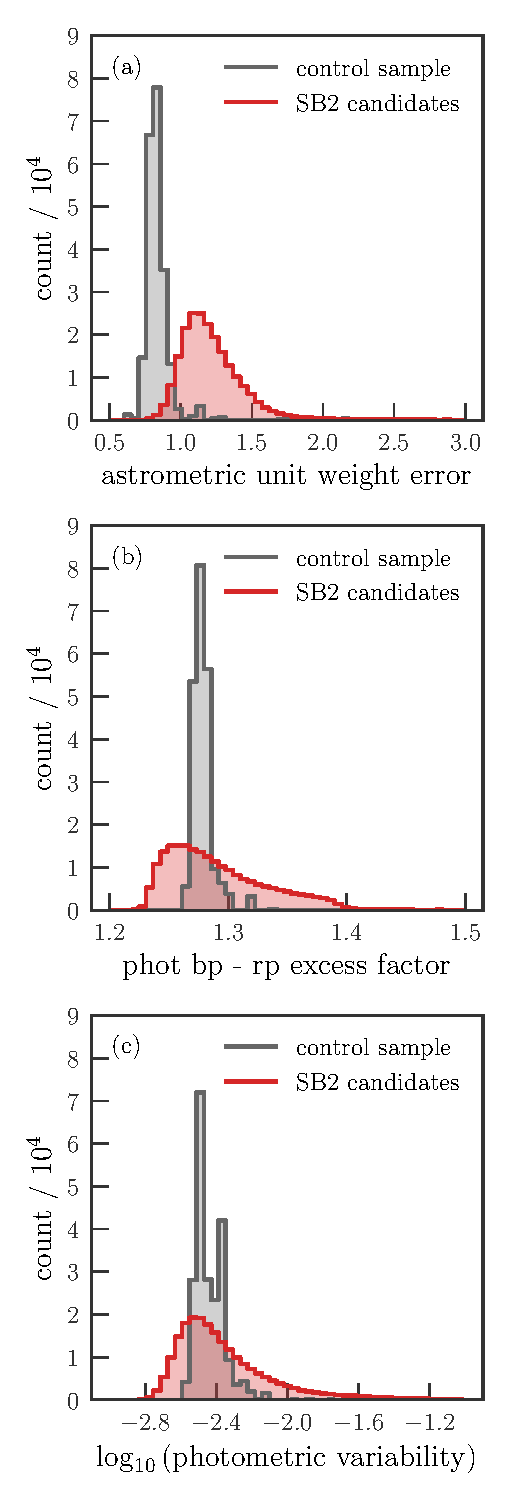
\includegraphics[width=0.4\textwidth]{../figures/sb2_histograms.pdf}
	
\includegraphics[width=0.4\textwidth]{../figures/todo.png}
    \caption{Distribution of 
    			(a) astrometric unit weight error (see Eq. \ref{eq:astrometric_unit_weight_error}),
			%$u = \left(\chi_{al}^2/(N_{al} - 5)\right)^{1/2}$
			%		where $\chi_{al}^2$ and $N_{al}$ is the astrometric goodness-of-fit and number 
			%		of observations in the along-scan direction, respectively (columns 
			%			\texttt{astrometric\_chi2\_al} and \texttt{astrometric\_n\_obs\_al}), 
				(b) photometric \bp\ - \rp\ excess factor, 				
	 				and 
				(c) photometric \rp\ variability (see Eq. \ref{eq:photometric_variability})
			of candidate SB2 type systems relative to a control sample of the same size.}
    \label{fig:sb2_histograms}
\end{figure}



% Figure: cross-match against a catalog of SB2 systems,... do we find all of
% 		  what they find from SB2 deductive inference alone? or do we miss
% 		  some SB2s in some parameter range?


%\subsection{Photometric binaries} \label{sec:method_photometric_binaries}

%\begin{eqnarray}
%	\textrm{Amp} = \log_{10}\left(\sqrt{N_{obs,al}}\frac{\sigma_{\langle{}f_G\rangle}}{\langle{}f_G\rangle}\right) \label{eq:photometric_variability}
%\end{eqnarray}




\section{Results} \label{sec:results}

\begin{figure}
	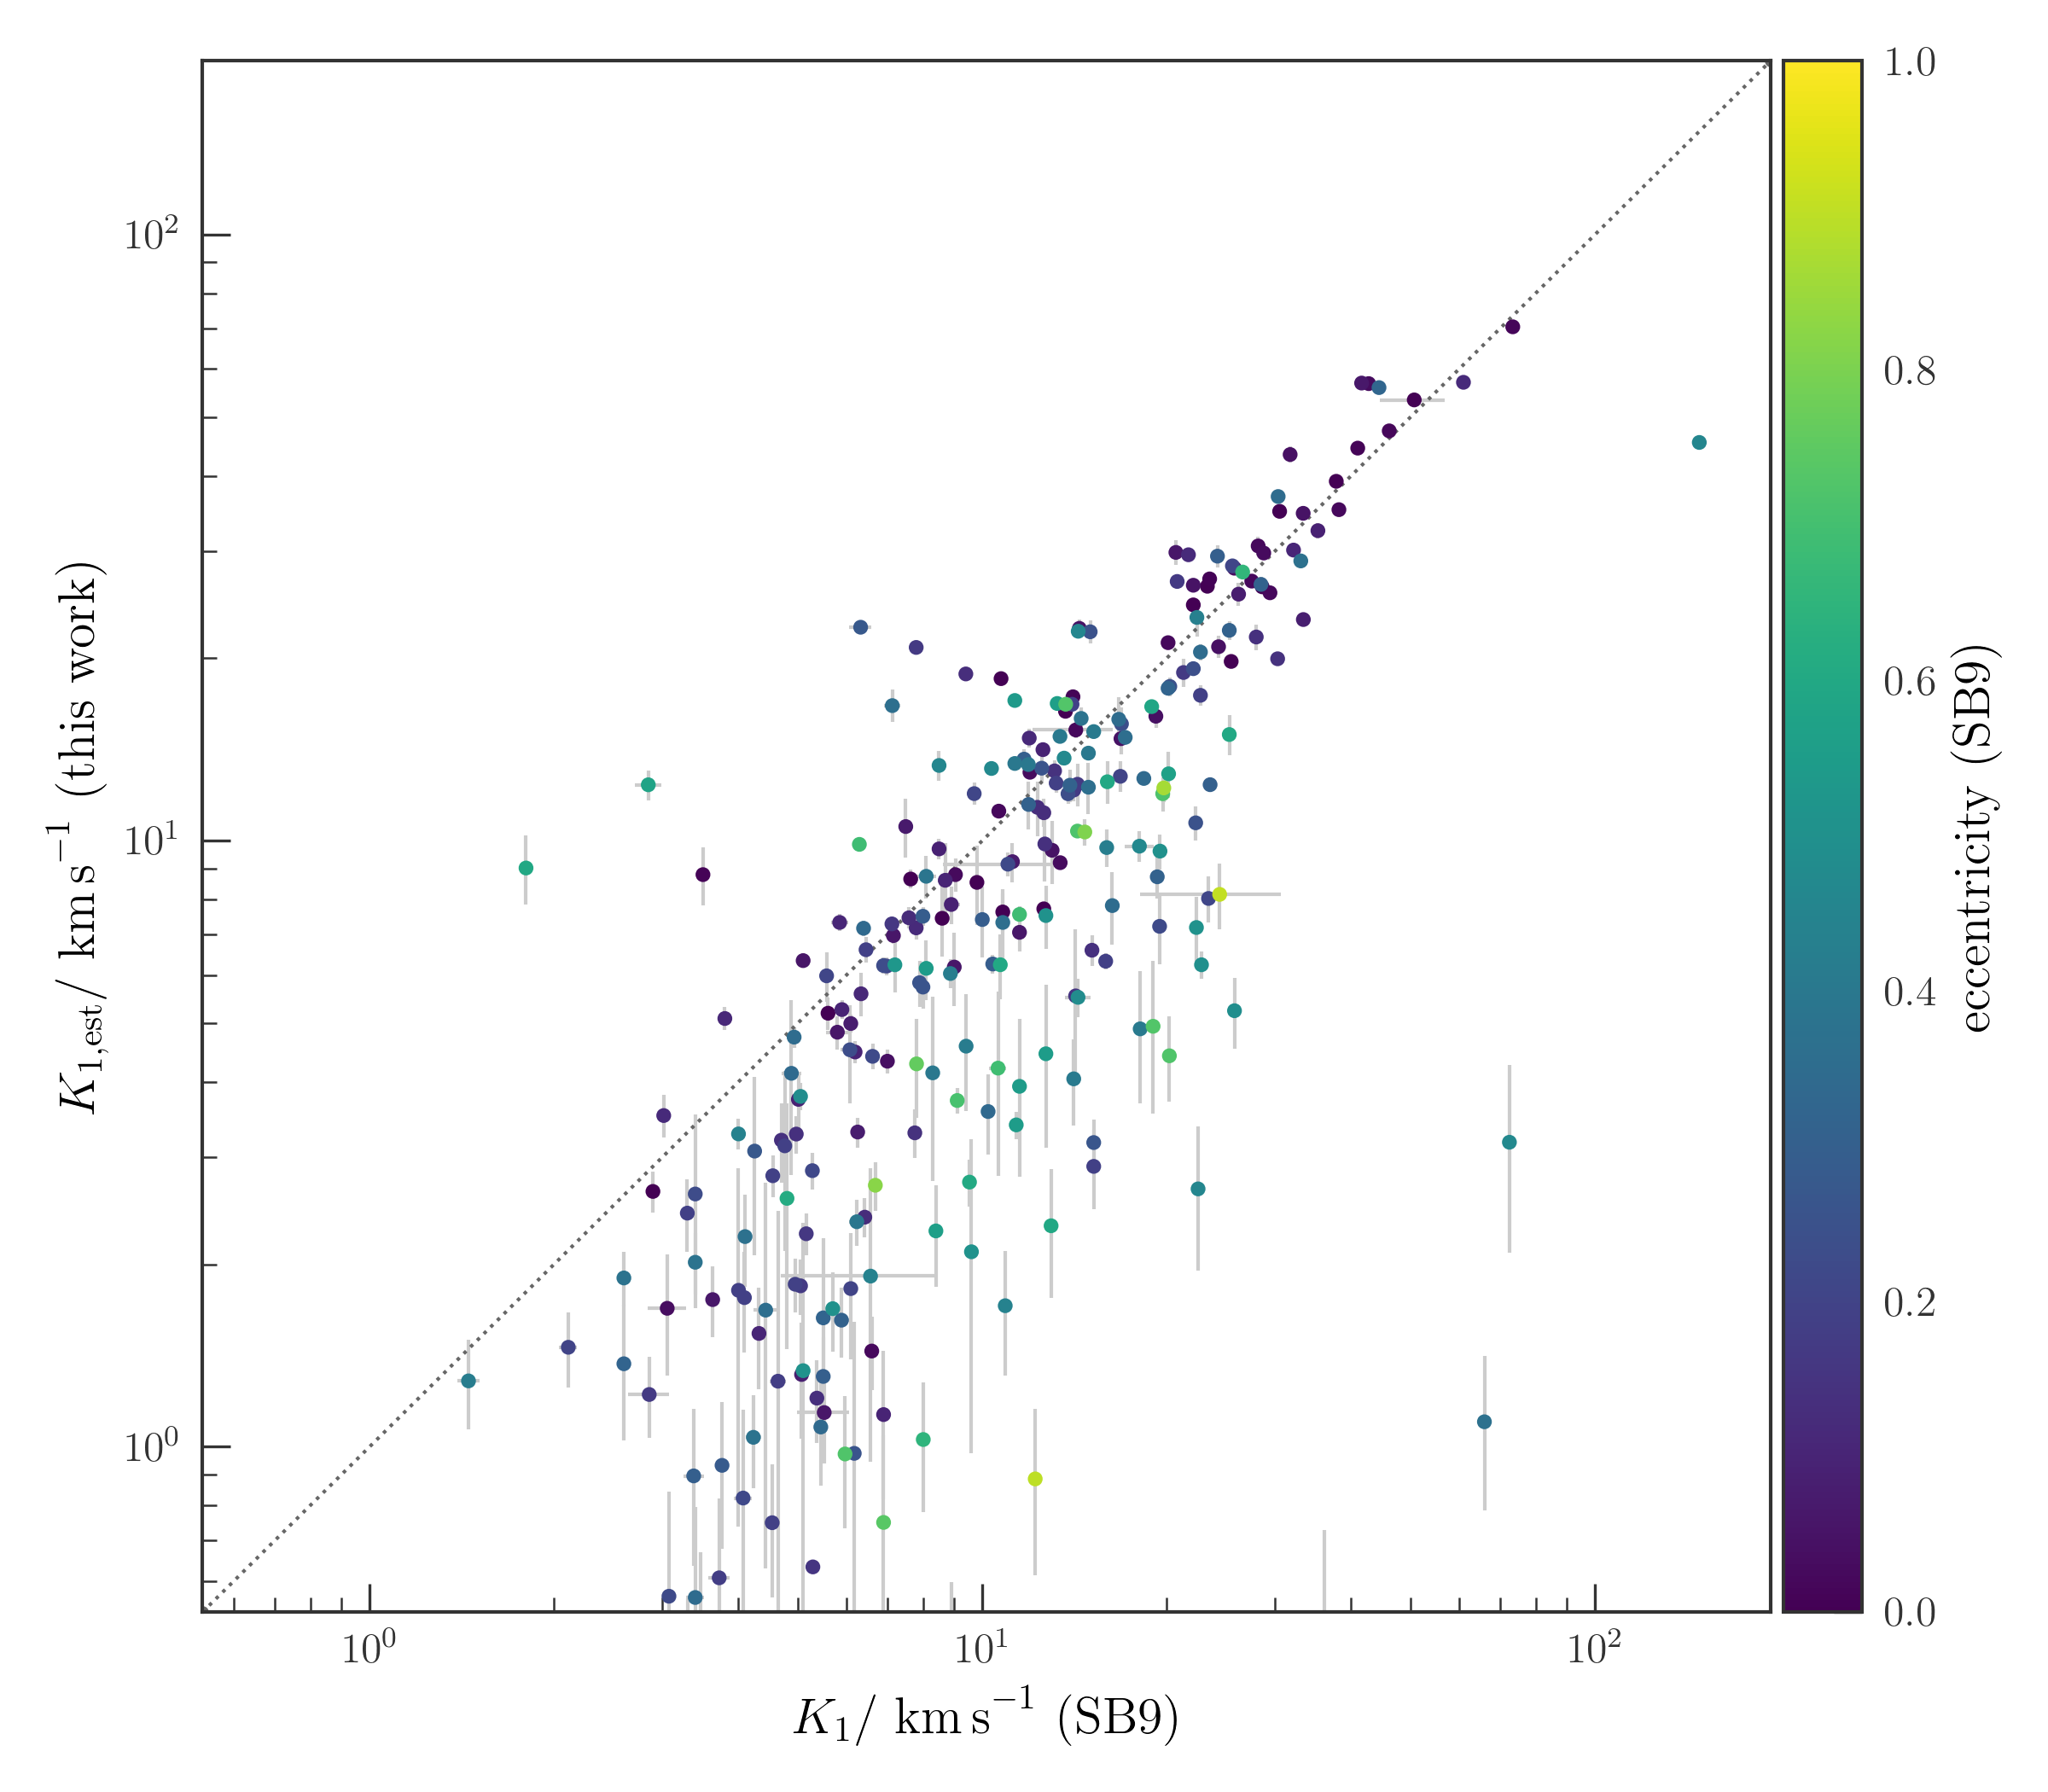
\includegraphics[width=0.5\textwidth]{figures/rv_sb9_k_comparison_v5.png}
    \caption{}
    \label{fig:rv_sb9_k_comparison}
\end{figure}

\begin{figure}
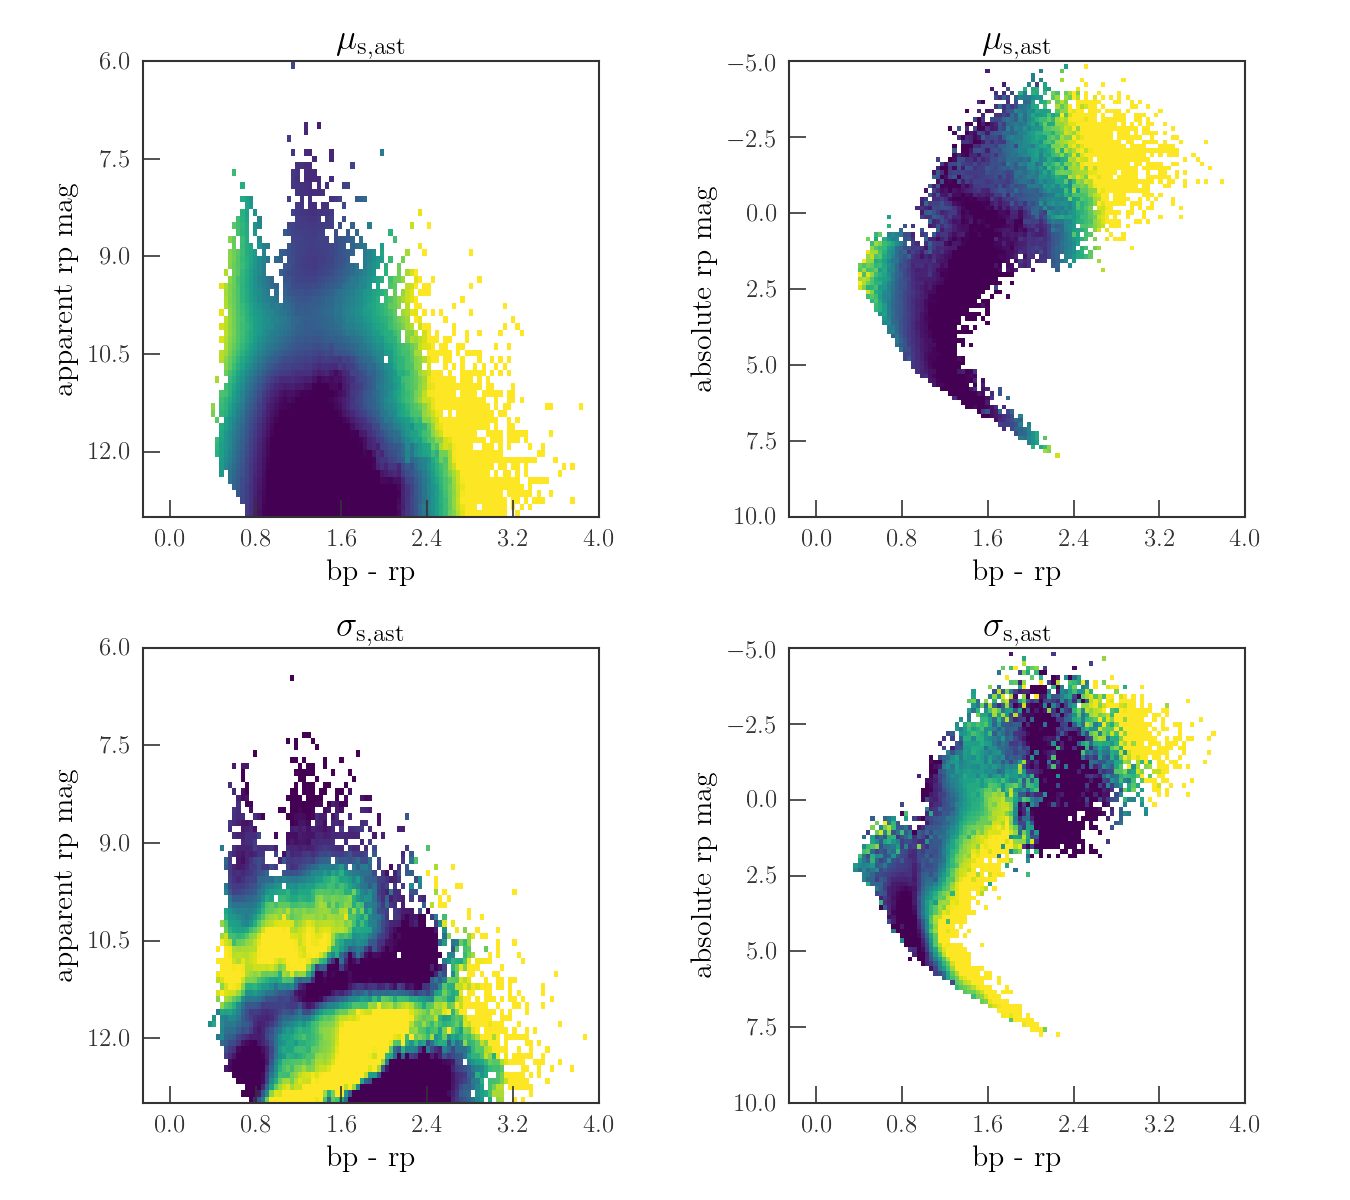
\includegraphics[width=0.5\textwidth]{figures/ast_gp_hrd_v5.png}
\caption{}
\label{fig:ast_gp_hrd_v5}
\end{figure}

\begin{figure}
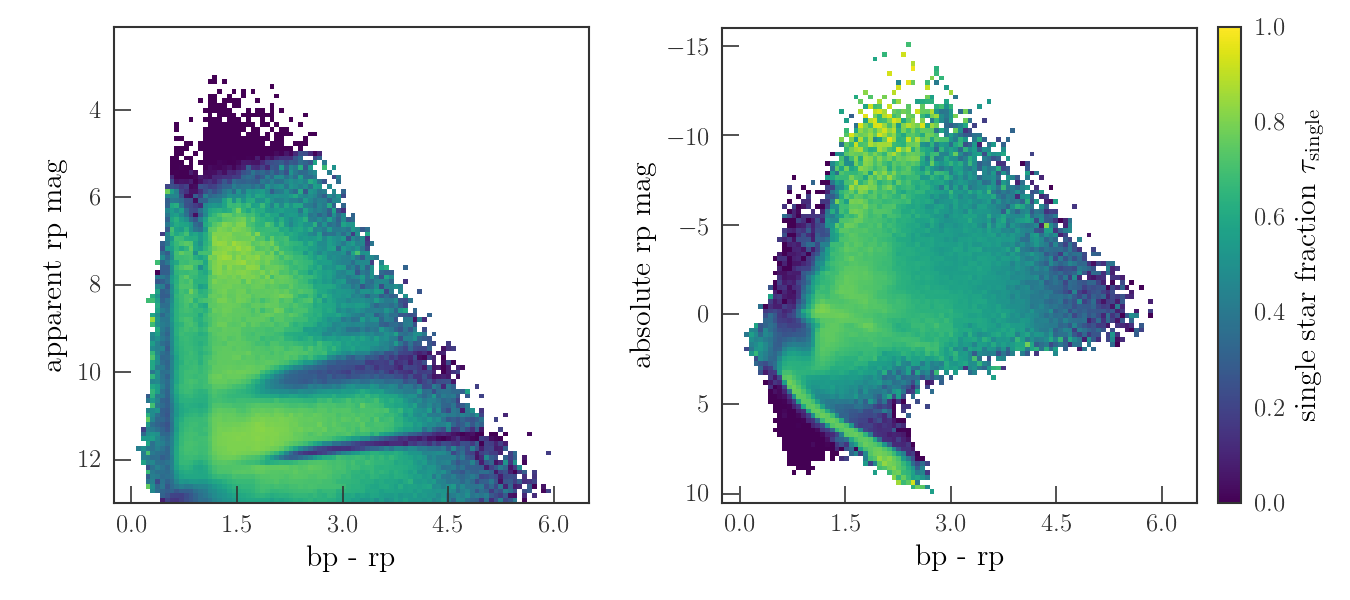
\includegraphics[width=0.5\textwidth]{figures/hrd_single_star_fraction_hist.png}
\caption{}
\label{fig:hrd_single_star_fraction_hist}
\end{figure}

\begin{figure}
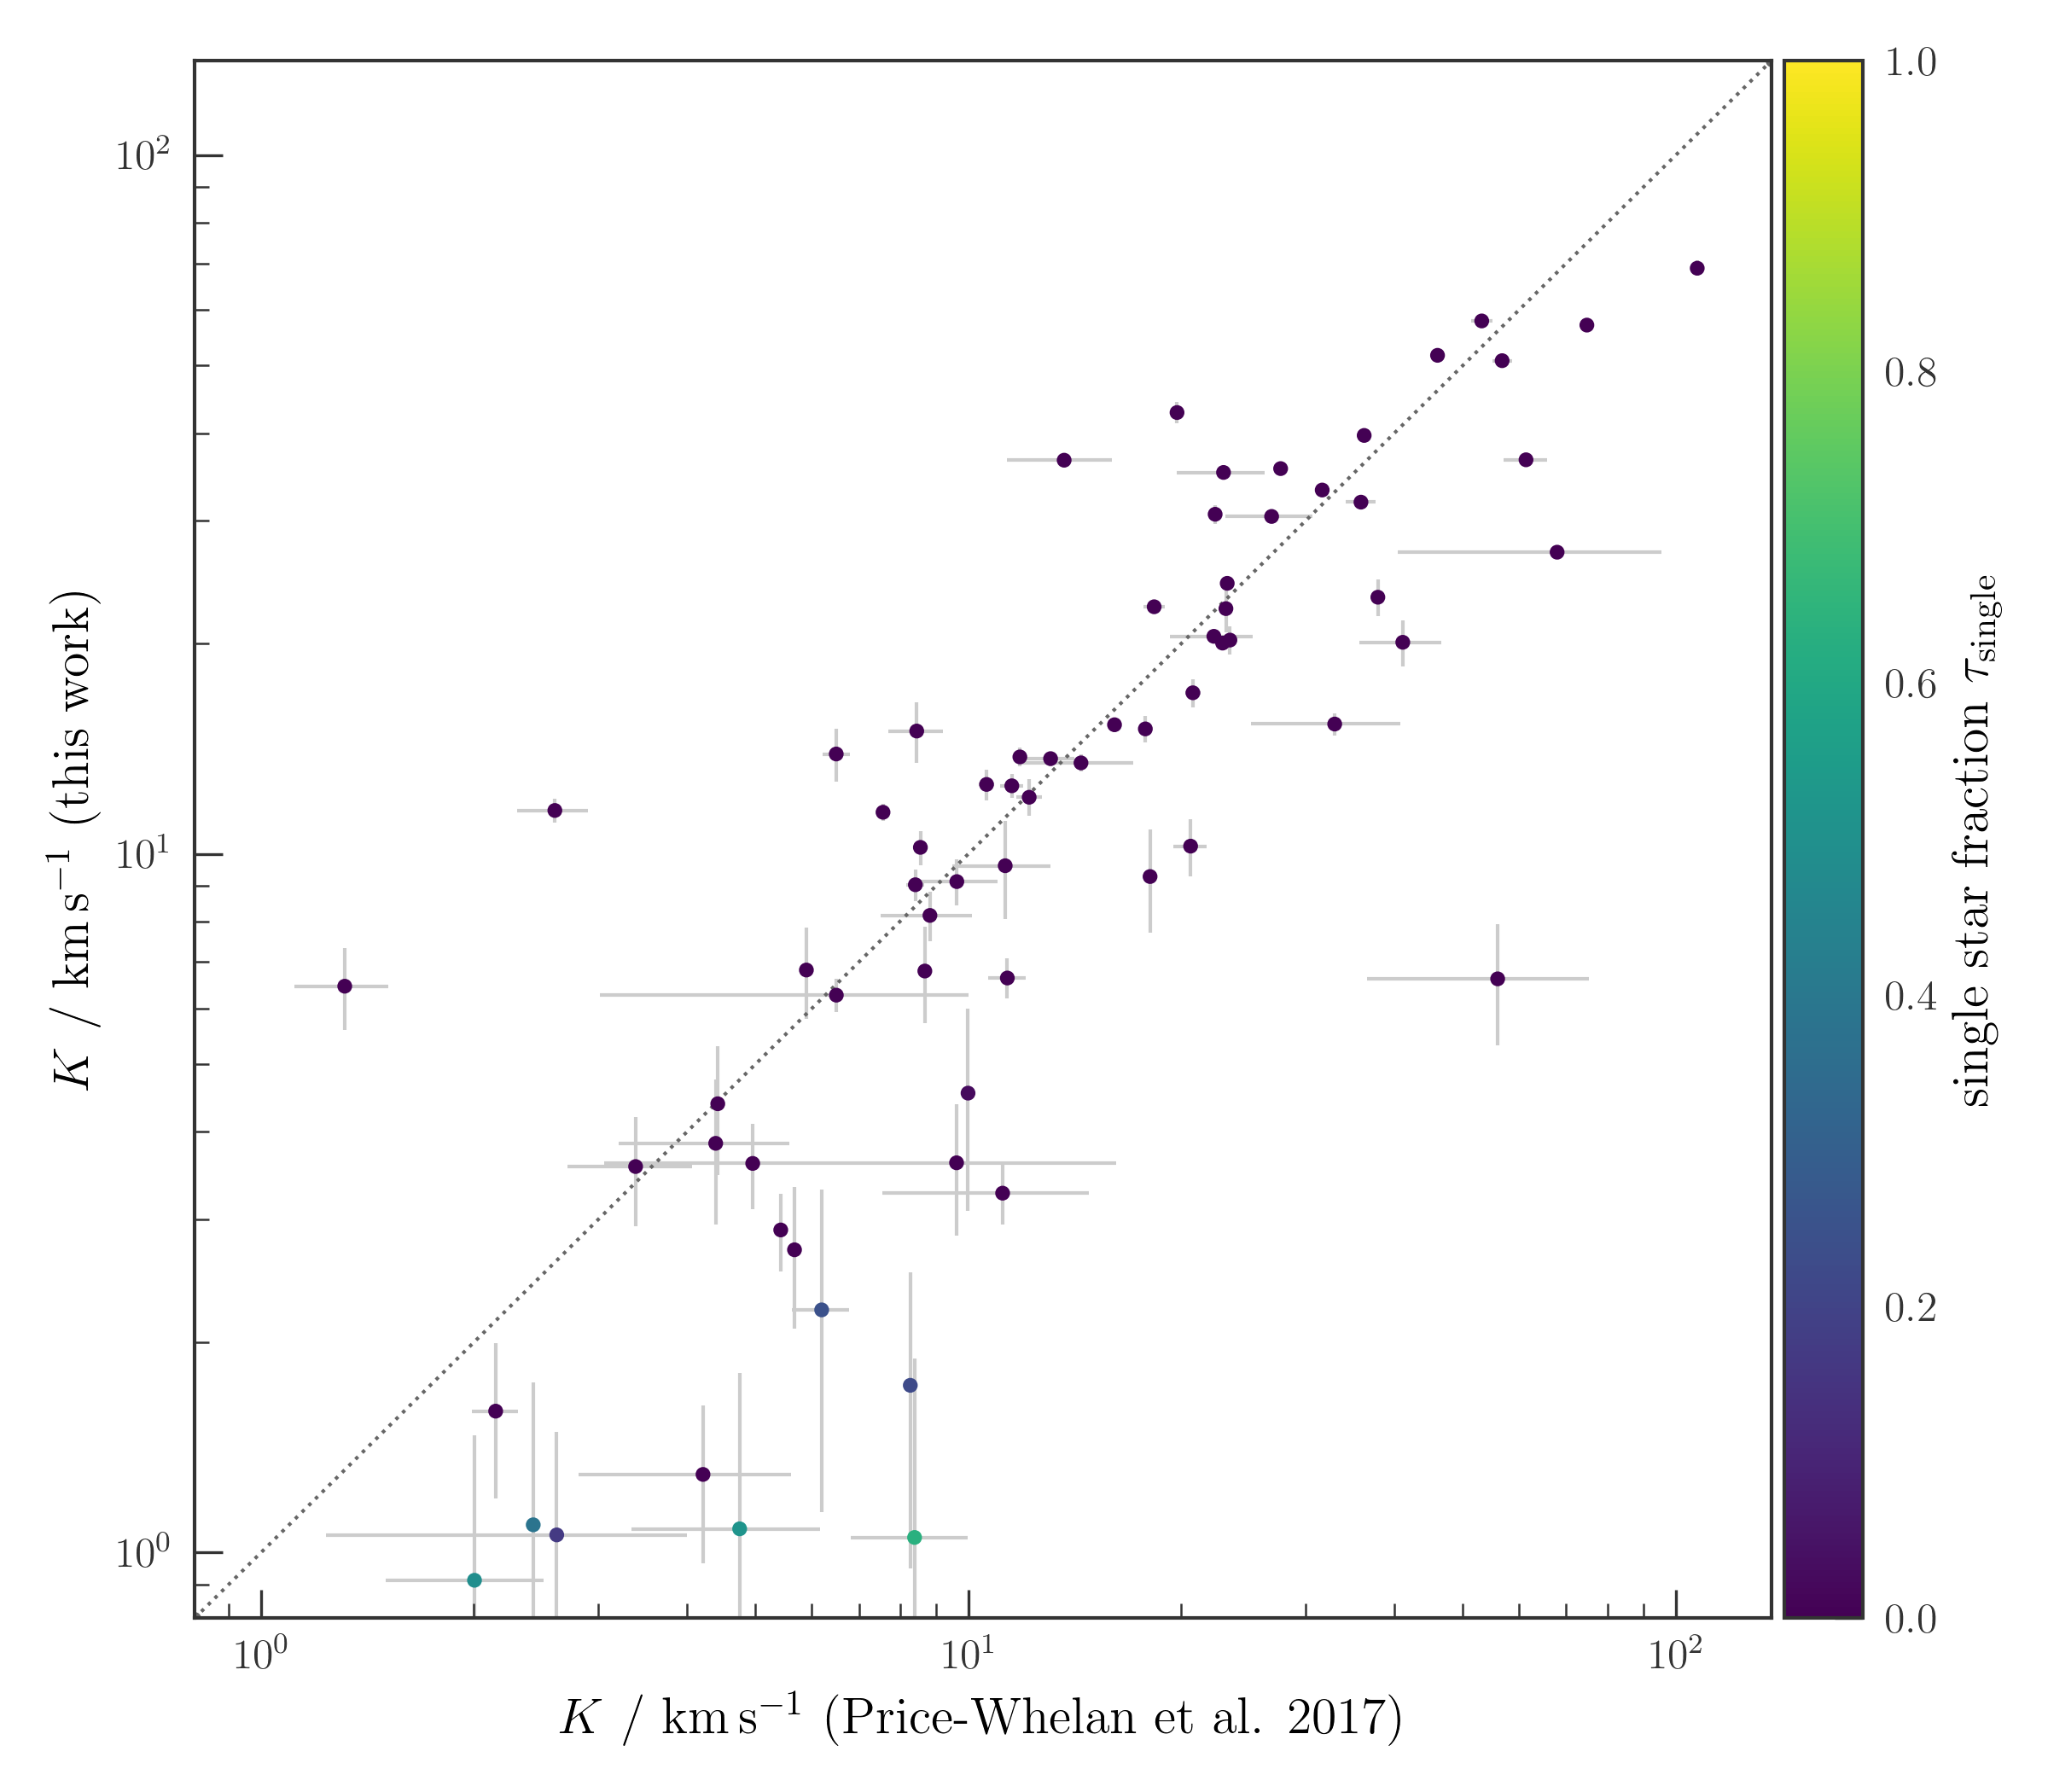
\includegraphics[width=0.5\textwidth]{figures/rv_apw_unimodal_k_comparison_v5.png}
\caption{}
\label{fig:rv_apw_unimodal_k_comparison_v5}
\end{figure}

\begin{figure}
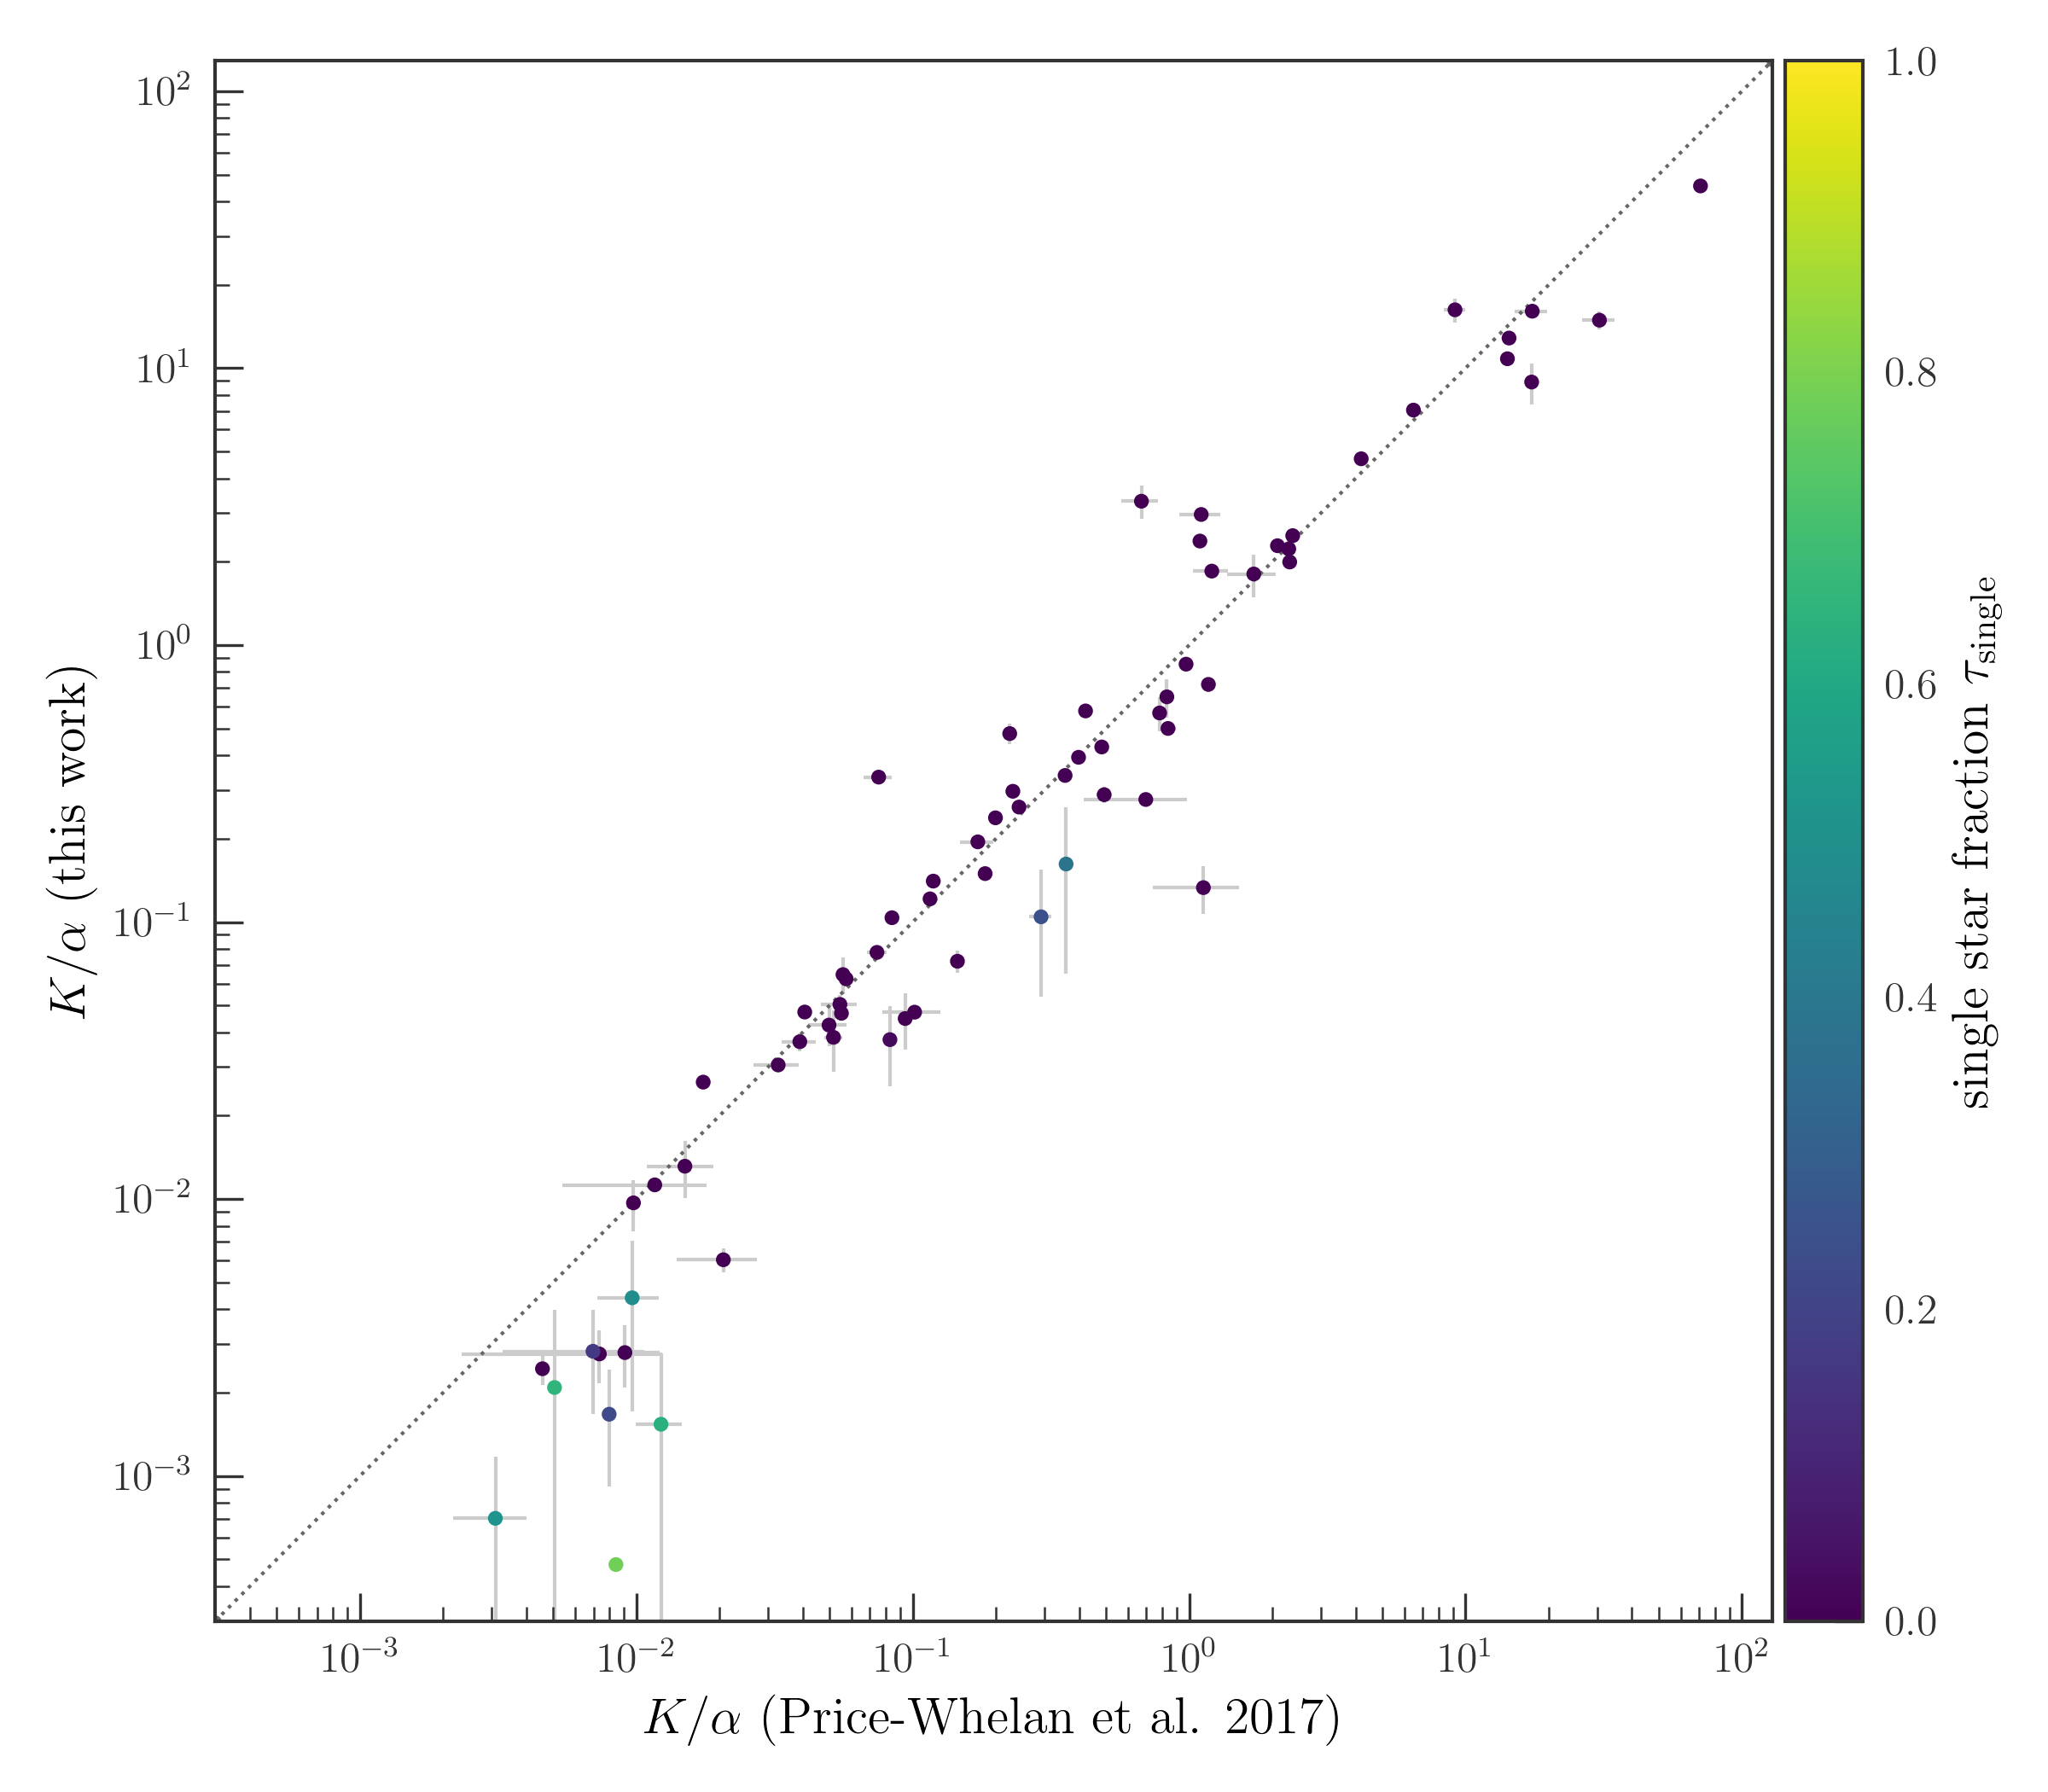
\includegraphics[width=0.5\textwidth]{figures/rv_apw_unimodal_kalpha_comparison_v5.png}
\caption{}
\label{fig:rv_apw_unimodal_kalpha_comparison_v5}
\end{figure}

\begin{figure}
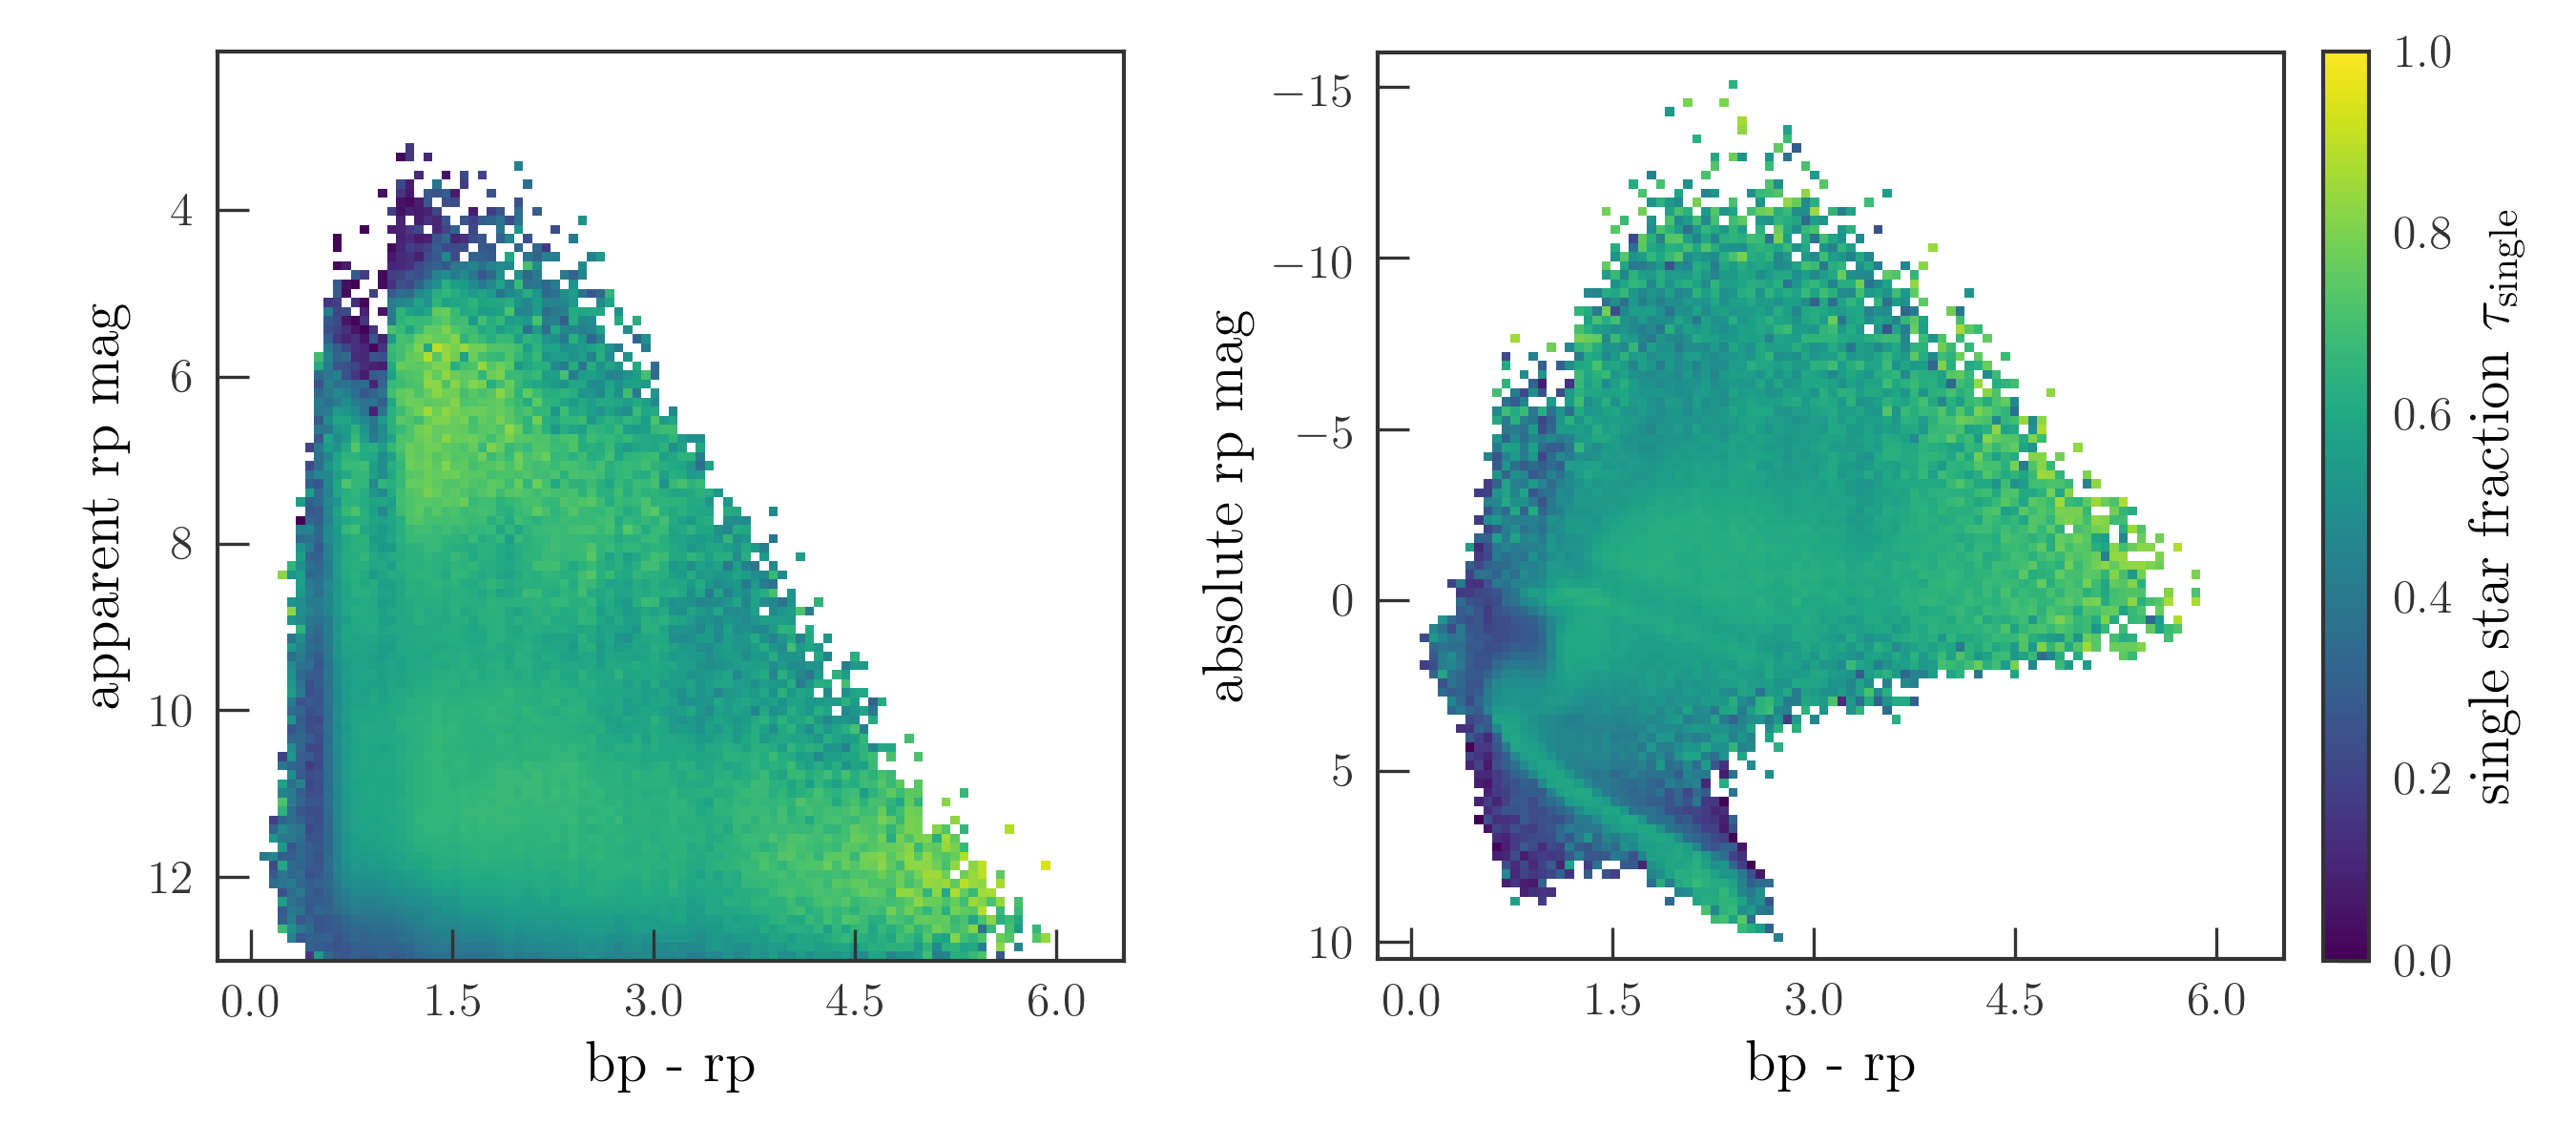
\includegraphics[width=0.5\textwidth]{figures/rv_hrd_single_star_fraction_hist_v5.png}
\caption{}
\label{fig:rv_hrd_single_star_fraction_hist_v5}
\end{figure}

\begin{figure}
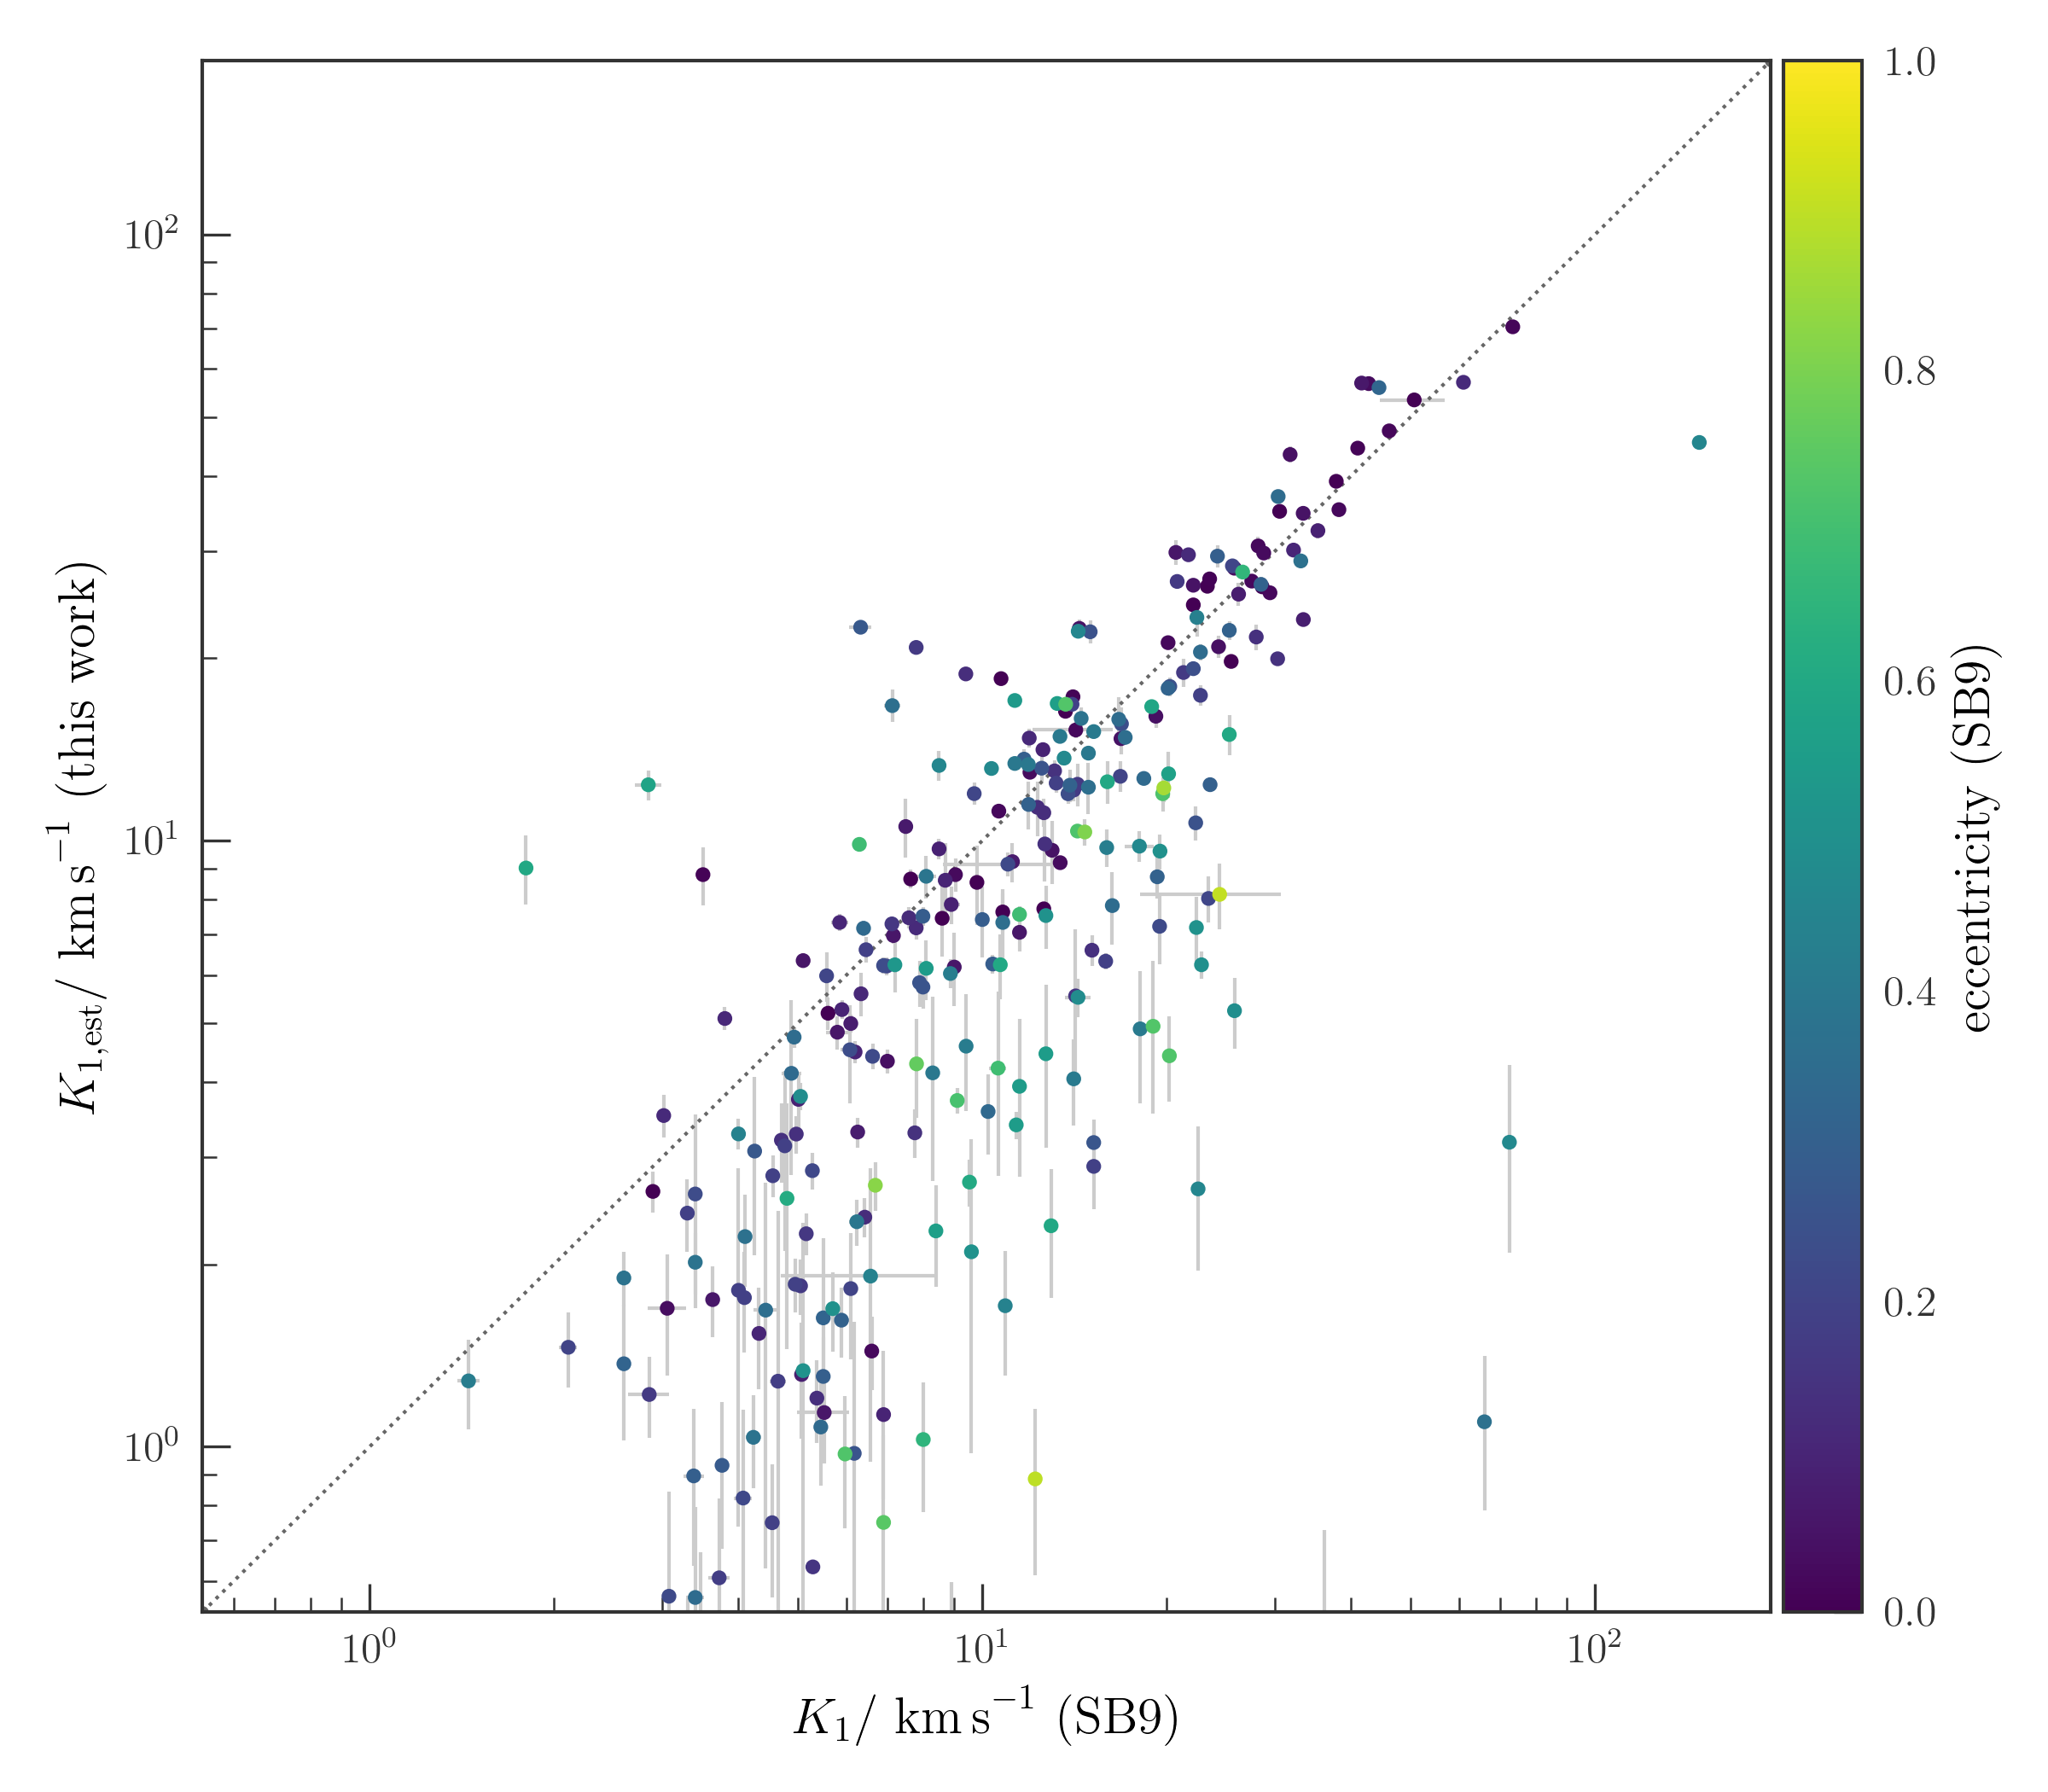
\includegraphics[width=0.5\textwidth]{figures/rv_sb9_k_comparison_v5.png}
\caption{}
\label{fig:rv_sb9_k_comparison_v5}
\end{figure}

\begin{figure}
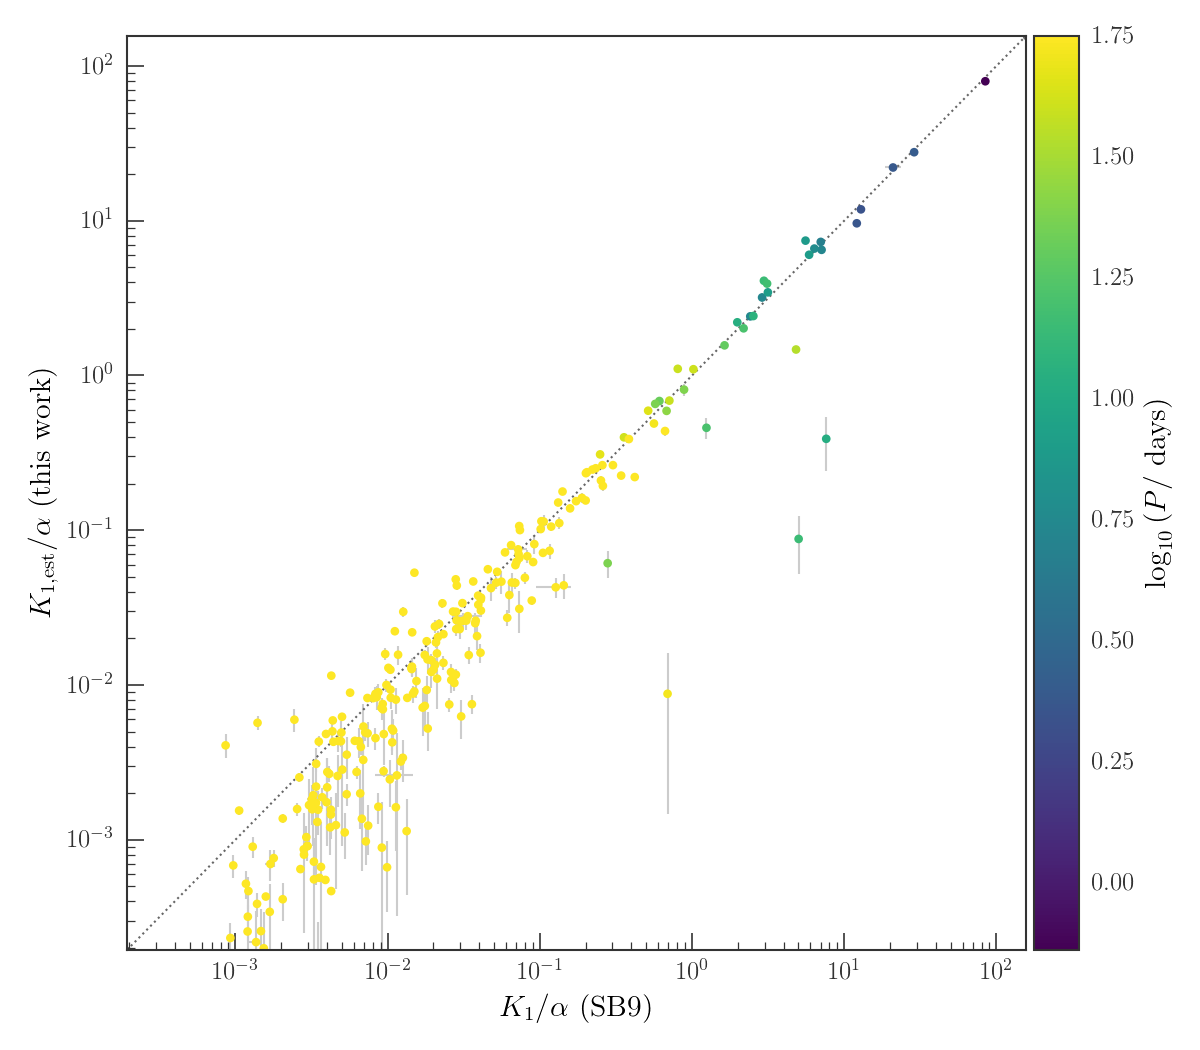
\includegraphics[width=0.5\textwidth]{figures/rv_sb9_kalpha_comparison_period.png}
\caption{}
\label{fig:rv_sb9_kalpha_comparison_period}
\end{figure}

\begin{figure}
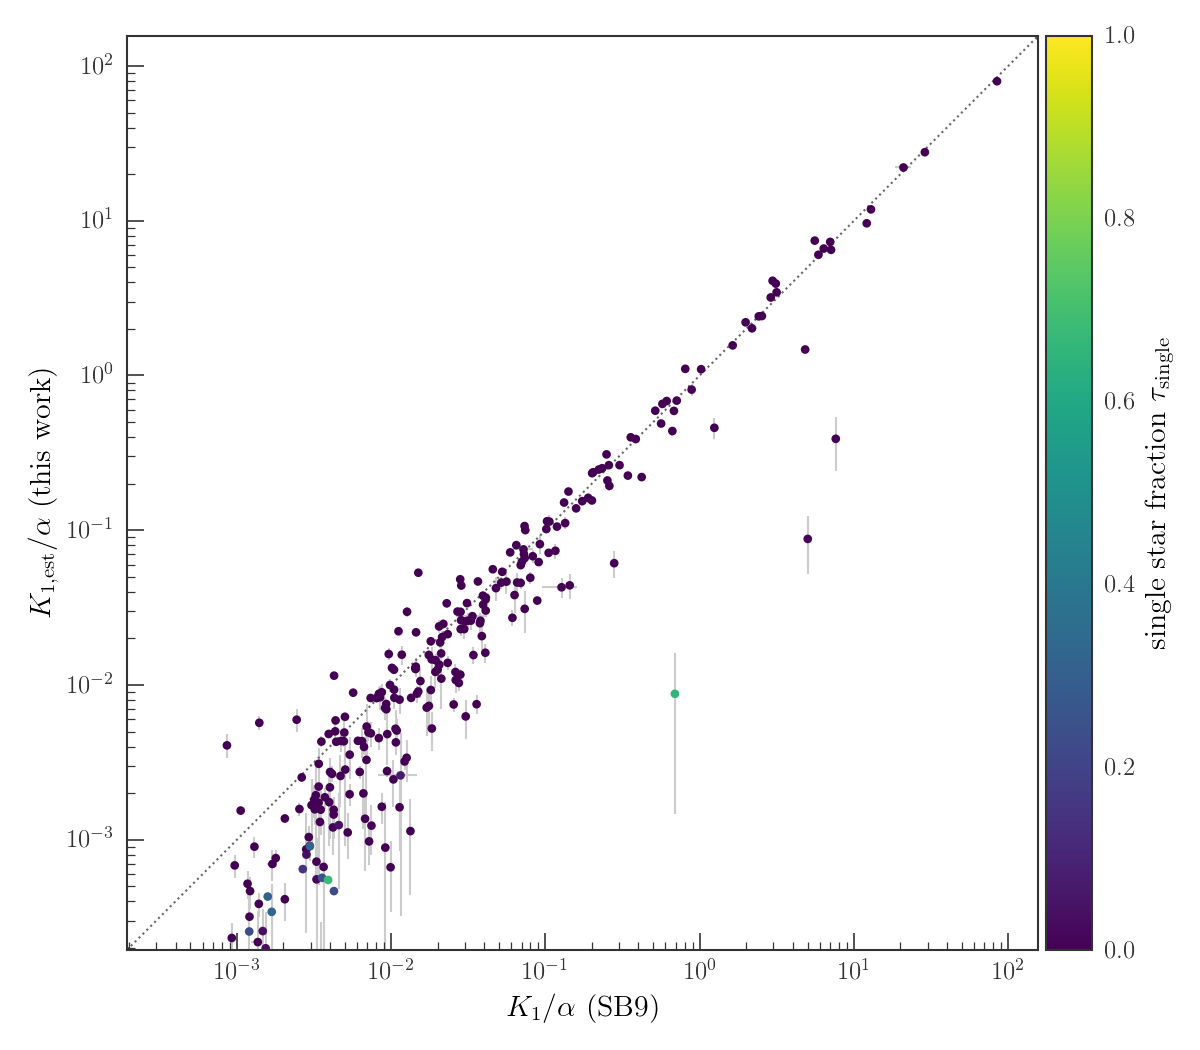
\includegraphics[width=0.5\textwidth]{figures/rv_sb9_kalpha_comparison_tau.png}
\caption{}
\label{fig:rv_sb9_kalpha_comparison_tau}
\end{figure}

\begin{figure}
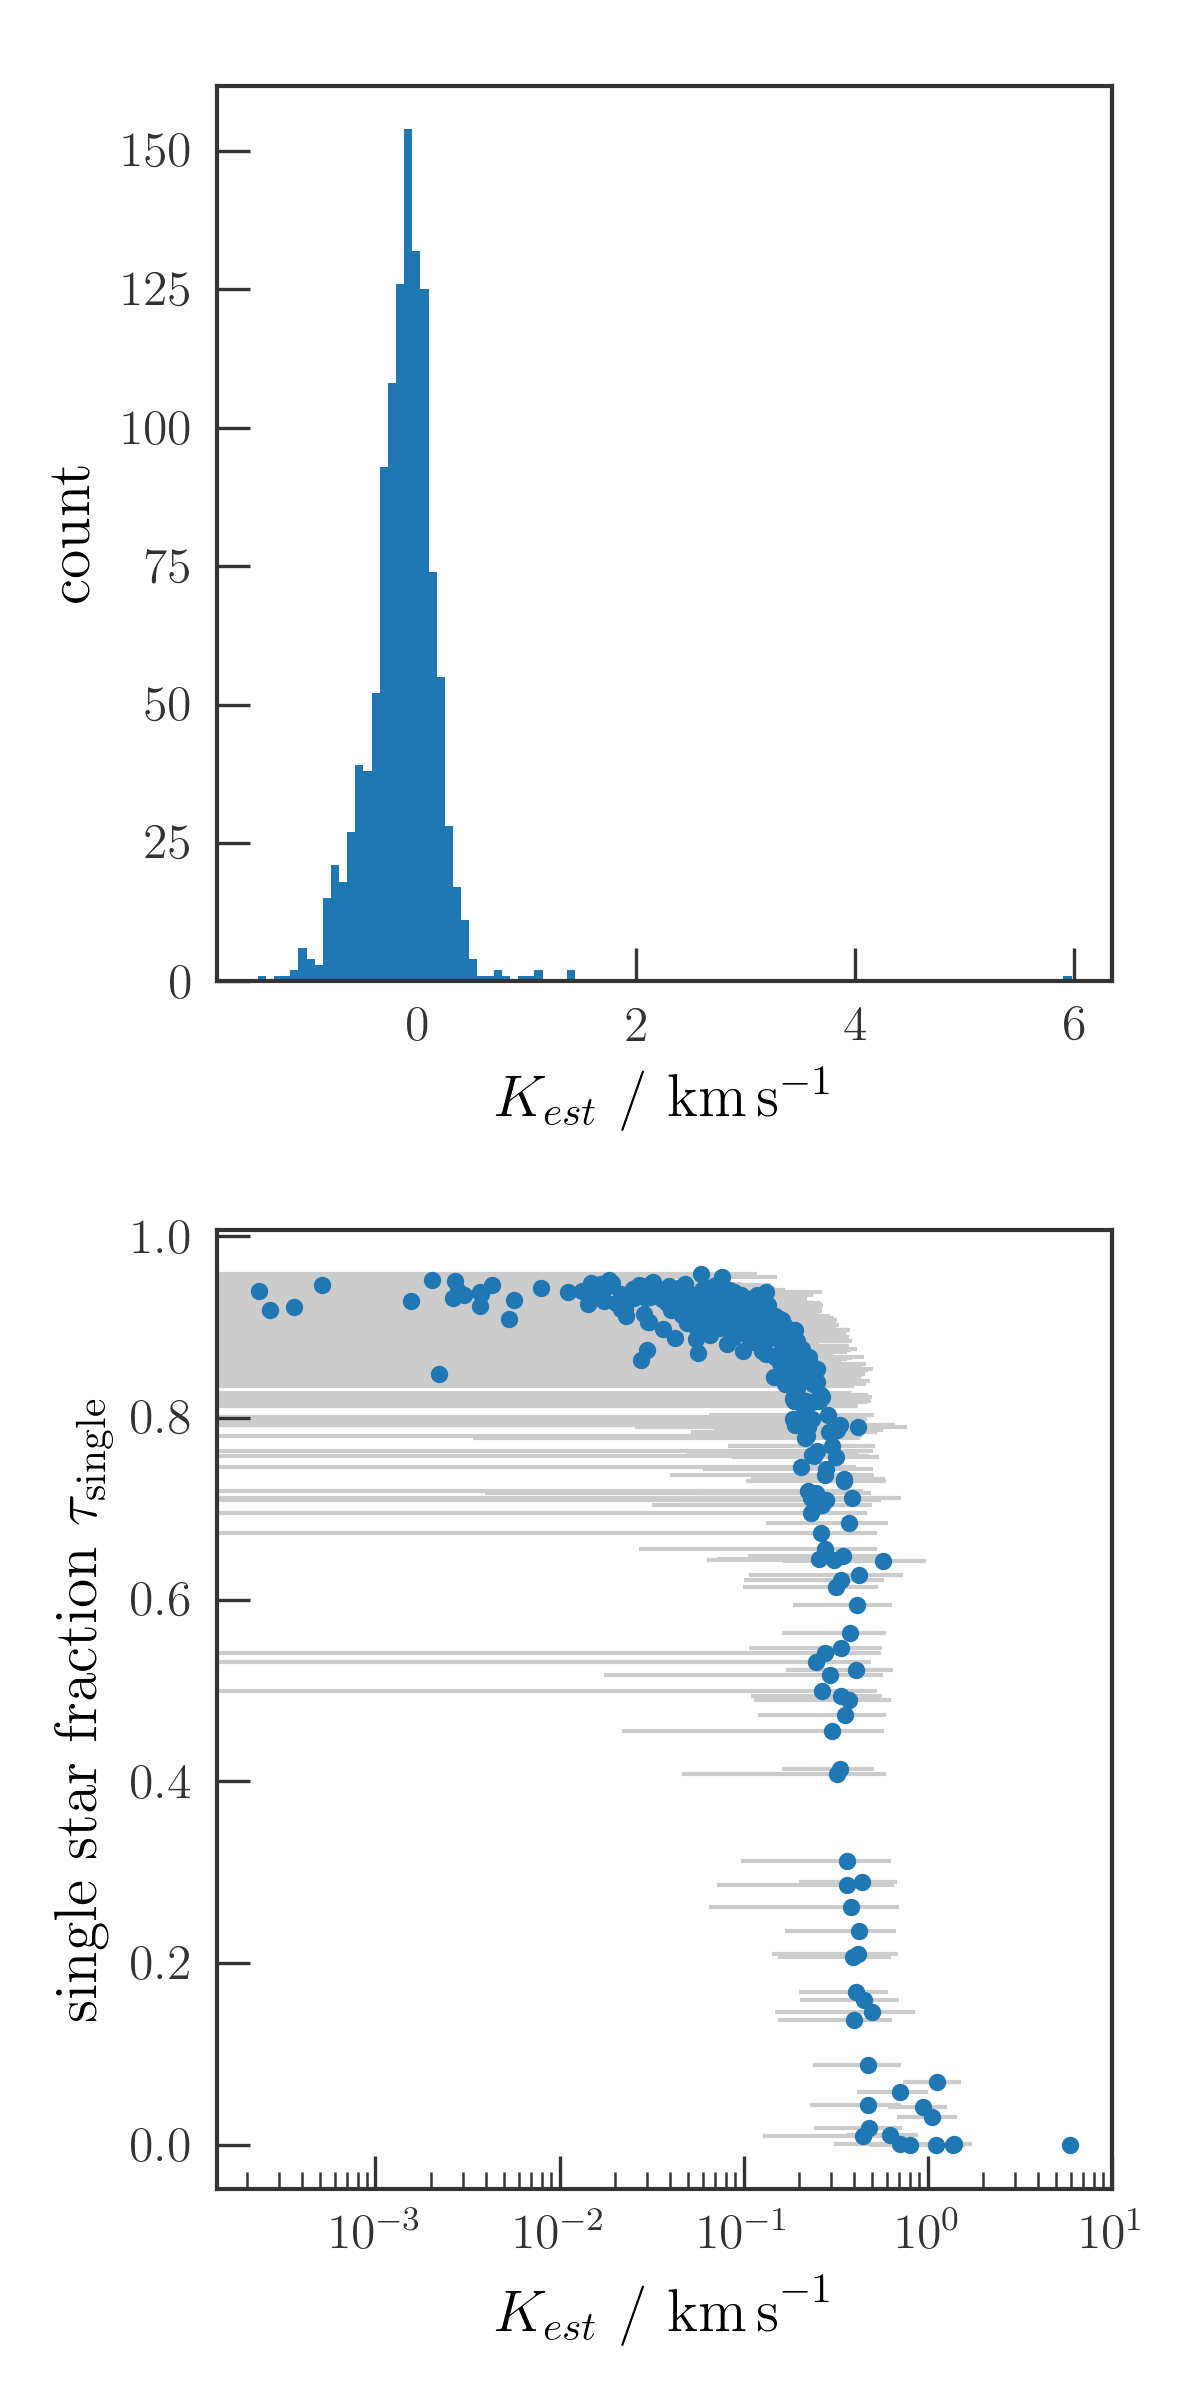
\includegraphics[width=0.5\textwidth]{figures/rv_soubiran_hist_v5.png}
\caption{}
\label{fig:rv_soubiran_hist_v5}
\end{figure}

\begin{figure}
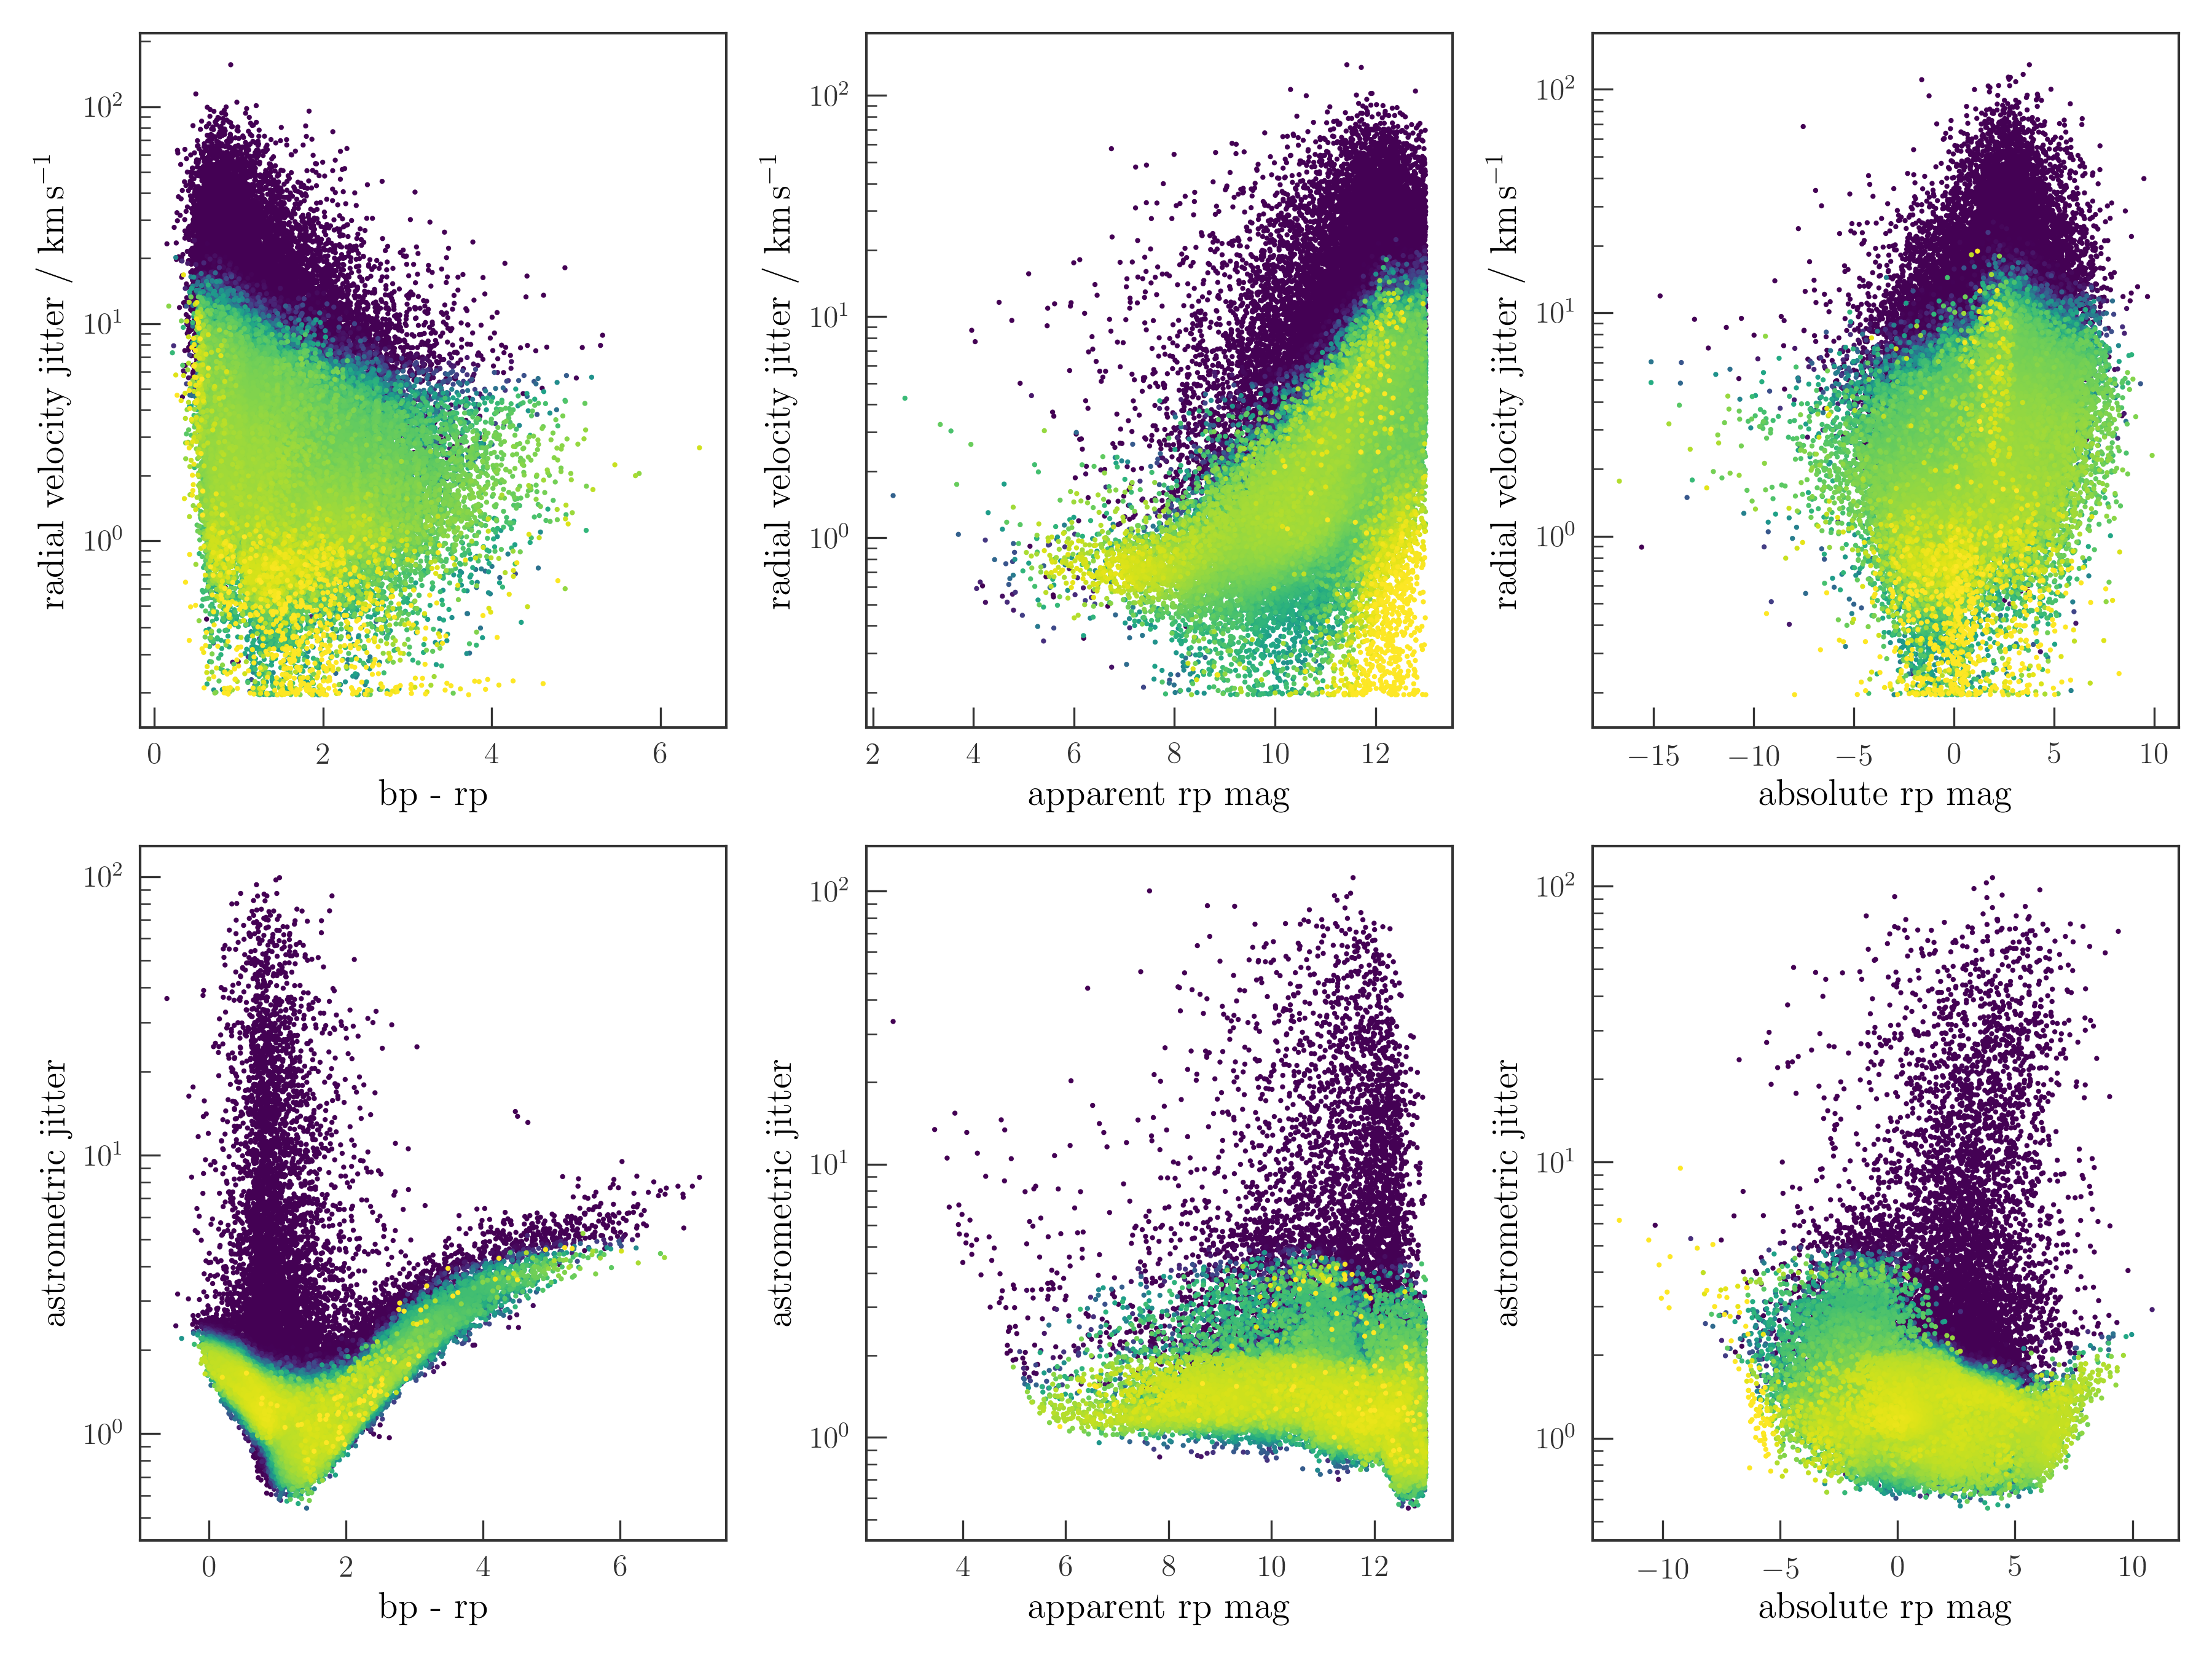
\includegraphics[width=0.5\textwidth]{figures/tau_single_wrt_kdt_labels_v5.png}
\caption{}
\label{fig:tau_single_wrt_kdt_labels_v5}
\end{figure}



\todo{We confirm that most stars are in binaries.}

- First convince the reader that we have measured something

- Comparisons: SB9, APW, et cetera

- Binary fraction as a  function  of everything

- Number of binaries detected as a function of things


\section{Discussion} \label{sec:discussion}


\begin{itemize}
	\item \todo{Binary fraction in the spaces that we were fitting: rp flux, colour, etc, just showing the transition of  probabilities}
	\item \todo{Binary fraction as a function of fitting properties (e.g., colour, absolute RP mag, apparent RP mag)}
	\item \todo{Binarity across the H-R diagram}
	\item \todo{What are the distributions of orbital parameters of binary systems that we would be able to detect?}
\end{itemize}

\subsection{Comparison with \citet{El-Badry:2018}}

\subsection{Comparison with \citet{Badenes:2018}}

\subsection{Comparison with \citet{Raghavan:2010}}

\subsection{Comparison with \citet{Troup:2016}}

\subsection{Comparison with \citet{Price-Whelan:2018}}

\begin{itemize}
	\item \todo{Binarity with metallicity }
    \item \todo{binarity in clusters vs the field?}
    \item \todo{binarity among extremely metal-poor stars?}
\end{itemize}


\acknowledgements

% At least some of these people will be promoted to the author list.
It is a pleasure to thank
	Berry Holl (Observatoire de Gen\'eve),
	Jose Hernandez (ESAC),
	Daniel Michalik (ESA/ESTEC),
	Kevin C. Schlaufman (Johns Hopkins University),
	Lorenzo Spina (Monash University),
		and
	Sergey Koposov (Carnegie Mellon University).
This work was supported in part by the Australian Research Council 
through Discovery Grant DP160100637.
This work has made use of data from the European Space Agency (ESA) mission {\it
Gaia} (\url{https://www.cosmos.esa.int/gaia}), processed by the {\it Gaia} Data
Processing and Analysis Consortium (DPAC,
\url{https://www.cosmos.esa.int/web/gaia/dpac/consortium}). Funding for the DPAC
has been provided by national institutions, in particular the institutions
participating in the {\it Gaia} Multilateral Agreement.  This research was
developed in part at the NYC Gaia DR2 Workshop at the Center for Computational
Astrophysics of the Flatiron Institute in 2018 April.

This work has made use of CosmoHub. CosmoHub has been developed by the Port 
d'Informaci\'o Cient\'ifica (PIC), maintained through a collaboration of the 
Institut de F\'isica d'Altes Energies (IFAE) and the Centro de Investigaciones 
Energ\'eticas, Medioambientales y Tecnol\'ogicas (CIEMAT), and was partially 
funded by the ``Plan Estatal de Investigaci\'on Cient�fica y T\'ecnica y de 
Innovaci\'on'' program of the Spanish government.


\appendix
\section{Reproducibility}
This project was developed in a \texttt{git} repository that is publicly
accessible at \giturl. The repository includes notebooks that detail our work,  
\LaTeX\ to compile this manuscript, and scripts to reproduce the results presented in
this manuscript. The results presented here can be reproduced in full (including data
retrieval, analysis, creation of figures, and manuscript compilation) using these
commands on a modern terminal:
% this is not python, but latex fails to evaluate \githash if I set bash environment.
\begin{minted}[
style=friendly,
escapeinside=||
]{python} 
git clone https://github.com/andycasey/velociraptor.git velociraptor
cd velociraptor
git checkout |\githash|
./reproduce
\end{minted}

Reproducing these results will require at least \todo{X}\,Gb of free disk space 
and \todo{Y}\,hours of compute time. The settings in \texttt{model.yaml} can be 
adjusted to reduce the sample size of the data and shorten the compute time, but
varying these settings does not guarantee exact replication of the results shown
here.


\section{Radial velocity completeness as a function of \Gaia\ source properties}



\subsection{SB2 Systems: Double-lined spectroscopic binaries}
\label{sec:sb2_methods}

Many sources in the second \Gaia\ data release do not have a reported radial 
velocity, despite being bright enough ($G \lesssim 13$) and in a suitable 
temperature range (e.g., between $\approx4000\,\textrm{K}$ and $\approx6500\,\textrm{K}$) 
for radial velocities to be measured \citep{Cropper:2018}. The principle reason 
why radial velocity measurements are \emph{not} reported for these stars is 
because the \Gaia/DPAC team have identified the source to be a double-lined 
spectroscopic binary (a so-called SB2-type system), either through a 
composition of two stellar sources present in the spectra, or from multiple 
(significant) modes in the cross-correlation function. In these situations it
is not sensible to report a point estimate of the radial velocity of the point 
source. For fainter or bluer sources, however, the radial velocity 
may not be reported simply because it is too faint, blue, or red. 


We calculated the completeness of radial velocity measurements (e.g., the
fraction of sources with reported radial velocities) as a function of all 
available source properties that might affect whether the radial velocity may
be reported or not. This included position ($\alpha$, $\delta$, $l$, $b$),
parallax, proper motions, apparent magnitudes, \bp\ - \rp\ colour, 
properties of the radial velocity templates, stellar parameters ($\teff$, $\radius$, $\luminosity$),
and other properties. The full list of properties investigated is described in
Appendix \ref{appendix:sb2}, with corresponding figures. 

In Figure \ref{fig:radial_velocity_completeness} we show the completeness as 
a function of some pertinent properties, which demonstrate that the radial 
velocity completeness is relatively flat until a source becomes too faint 
(low \rp\ flux), or is either too blue or too red. We adopt conservative 
limits for when the radial velocity completeness starts to drop with these 
properties, and we assume that any source within the following range of 
source parameters
\begin{eqnarray}
    \mathrm{phot\,\,rp\,\,mean\,\,flux} & \in & [10^{4}, 10^8] \nonumber \\
    \mathrm{bp-rp} & \in & [X, Y] 
    \label{eq:sb2_criteria}
\end{eqnarray}
\noindent{}is likely to be a double-lined spectroscopic binary (SB2) if no 
radial velocity is reported. That is to say that we are explicitly assuming
that if a point source meets the criteria in Equation \ref{eq:sb2_criteria} 
and does not have a reported radial velocity measurement, then the point 
source is an unresolved double-lined spectroscopic binary. In principle we 
could make more realistic attempts to model the radial velocity completeness as
a function of stellar properties rather than simply stating ``sources within
this parameter range should have radial velocities unless they are SB2 systems'',
but the radial velocity completeness within our specified range is reasonably
flat.


\todo{Some confirmation of this? The properties of SB2 candidate systems relative to others. Figure \ref{fig:sb2_histograms}.}


We stress that our sample of SB2 type systems is calculated (or rather, deduced)
separately to our calculations of multiplicity probability given the 
\emph{measured} quantities from \Gaia\ like radial velocity, astrometry, and
photometry. In Section \ref{sec:discussion} we detail some of the immediate
limitations or interpretations of this assumption, and we emphasise that the 
main conclusions of this work do not depend on SB2 systems. Nevertheless, we 
\emph{strongly} 
caution that our deductive inference of SB2 systems will be far more uncertain 
than the binary probabilities we derive from other information. Our indicator 
whether a star is likely a SB2 system likely suffers from more contamination
and lower completeness compared to the probabilities we derive from other information
(e.g., the radial velocity jitter, astrometric excess noise, and photometric 
colours), and the contamination and completeness likely vary over some
complex (unknown) function of parameter space. 




\begin{figure*}
%	\includegraphics[width=1.0\textwidth]{../figures/sb2_rvs_completeness.pdf}
	
\includegraphics[width=1.0\textwidth]{../figures/todo.png}
    \caption{Fraction of \Gaia\ sources with reported radial velocities
		     as a function of source properties. Within the adopted source
		     parameter ranges (gray; see Section \ref{sec:sb2_methods})
		     the radial velocity completeness is approximately flat.
		     We flag sources within this range that do not have reported 
		     radial velocities to be candidate SB2 systems.}
    \label{fig:sb2_rvs_completeness}
\end{figure*}




\begin{figure*}
%	\includegraphics[width=1.0\textwidth]{../figures/sb2_sky_structure.pdf}
	
\includegraphics[width=1.0\textwidth]{../figures/todo.png}

    \caption{Fraction of sources (per sky bin) without reported radial velocities
    		 for all sources with $G \lesssim 13$ (top) and sources in the ranges
		 	 specified by Eqs \ref{eq:sb2_ranges} (bottom), where we assert that a missing
			 radial velocity measurement signifies a likely SB2 candidate . The color scale is 
			 arbitrarily set to highlight structure, where black indicates a higher
			 fraction of sources do not have reported radial velocities. Crowding
			 in the galactic plane likely results in some sources not having radial
			 velocities reported. The large scale structure visible in both axes is
			 a combined effect of the initial \Gaia\ source list, the scanning law,
			 and star forming regions (i.e., where emission in the \ion{Ca}{2} 
			 triplet likely causes issues for radial velocity determination).}
    \label{fig:sb2_sky_structure}
\end{figure*}



% astroquery
% minted
\software{
	\package{Astropy} \citep{astropy:v1,astropy:v2},
    \package{IPython} \citep{ipython},
    \package{matplotlib} \citep{mpl},
    \package{numpy} \citep{numpy},
    \package{scipy} \citep{scipy},
    \package{Stan} \citep{stan},
    \package{CosmoHub} \citep{cosmohub},
    \package{TensorFlow} \citep{tensorflow}
    \package{Jupyter Notebooks} \citep{jupyter-notebooks}
}    

\bibliographystyle{aasjournal}
\bibliography{velociraptor}

\end{document}
